\section{(4) Определение графа, графов с петлями и кратными ребрами. Ориентированные графы. Лемма
о рукопожатиях. Четыре определения дерева и их эквивалентность.}
\section{Асимптотические обозначения: $O, \Omega, \Theta$. Независимость от стартового индекса. Мастер-теорема (б/д).}
\par \textbf{Определение:} Пусть $f,g: \; \mathbb{N} \rightarrow \mathbb{N}$. Тогда $f=O(g)$, если существует $c, N$, такие что $\forall n \in N \; \hookrightarrow n \geqslant N \Rightarrow f(n) \leqslant c \cdot g(n)$.
\par \textbf{Определение:} Пусть $f,g: \; \mathbb{N} \rightarrow \mathbb{N}$. Тогда $f=\Omega(g)$, если существует $c, N$, такие что $\forall n \in N \; \hookrightarrow n \geqslant N \Rightarrow f(n) \geqslant c \cdot g(n)$.
\par \textbf{Замечание:} $f = \Omega(g) \Leftrightarrow g = O(f)$
\par \textbf{Определение:} Пусть $f,g: \; \mathbb{N} \rightarrow \mathbb{N}$. Тогда $f=\Theta(g)$, если существует $c_1,c_2, N$, такие что $\forall n \in N \; \hookrightarrow \\ n \geqslant N \Rightarrow c_1 \cdot g(n) \leqslant f(n) \leqslant c_2 \cdot g(n)$.
\par \textbf{Замечание:} $f = \Theta(g) \Leftrightarrow f = O(g)$ и $f = \Omega(g)$
\par \textbf{Утверждение:} $f = O(g) \Leftrightarrow \exists c: \forall n \in \mathbb{N} \hookrightarrow f(n) \leqslant c \cdot g(n)$ 
\par \begin{itemize}
    \item[$\blacktriangle \Leftarrow$] Очевидно, достаточно положить $N=1$
    \item[$\Rightarrow$] Пусть $\forall n \geqslant N \hookrightarrow f(n) \leqslant c \cdot g(n)$. Определим $c'=\max \{c, \frac{f(1)}{g(1)}, \ldots, \frac{f(N)}{g(N)}\}$ ($g$ не обращается в 0 так как результат натуральный). Тогда \begin{enumerate}
        \item $n \geqslant N \Rightarrow f(n) \leqslant c \cdot g(n) \leqslant c' \cdot g(n)$
        \item $n < N \Rightarrow c' \geqslant \frac{f(n)}{g(n)} \Rightarrow f(n) \leqslant c' \cdot g(n) \; \blacksquare$
    \end{enumerate}
\end{itemize}
\par Для $\Omega$ и $\Theta$ справедливы аналогичные утверждения.
\par \textbf{Мастер-теорема (с лекции):} Пусть $T: \mathbb{N} \rightarrow \mathbb{N}$ с условием $T(n)=a \cdot T(\frac{n}{b})+f(n)$, $a=const, a \geqslant 1; \\ b=const, b \geqslant 1, f: \mathbb{N} \rightarrow \mathbb{N}$. Тогда \begin{enumerate}
    \item Если $\exists \varepsilon > 0$, такое что $f(n)=O(n^{\log_b a - \varepsilon})$, то $T(n)=\Theta(n^{\log_b a})$
    \item Если $f(n)=\Theta(n^{\log_b a})$, то $T(n)=\Theta(n^{\log_b a} \log n)$
    \item Если $\exists \varepsilon > 0$, такое что $f(n)=\Omega(n^{\log_b a + \varepsilon})$, причем $\exists c < 1$, такое что $a \cdot f(\frac{n}{b}) \leqslant c \cdot f(n)$ для всех $n$, начиная с некоторого номера, то $T(n)=\Theta(f(n))$
\end{enumerate}
\par \textbf{Мастер-теорема (из интернета):} Пусть имеется рекуррентное соотношение:
$$T(n)=\left\{
\begin{array}{ccc}
a \cdot T(\frac{n}{b})+O(n^c), n>1\\
O(1),n=1\\
\end{array}
\right., \text{ где } a \in \mathbb{N}, b \in \mathbb{R}, b>1, c \in R^+.$$

Тогда асимптотическое решение имеет вид: \begin{enumerate}
    \item Если $c>\log_b a$, то $T(n)=O(n^c)$
    \item Если $c=\log_b a$, то $T(n)=O(n^c \log n)$
    \item Если $c<\log_b a$, то $T(n)=O(n^{\log_b a})$
\end{enumerate}
\newpage{}

\section{(5) Код Прюфера. Формула Кэли.}
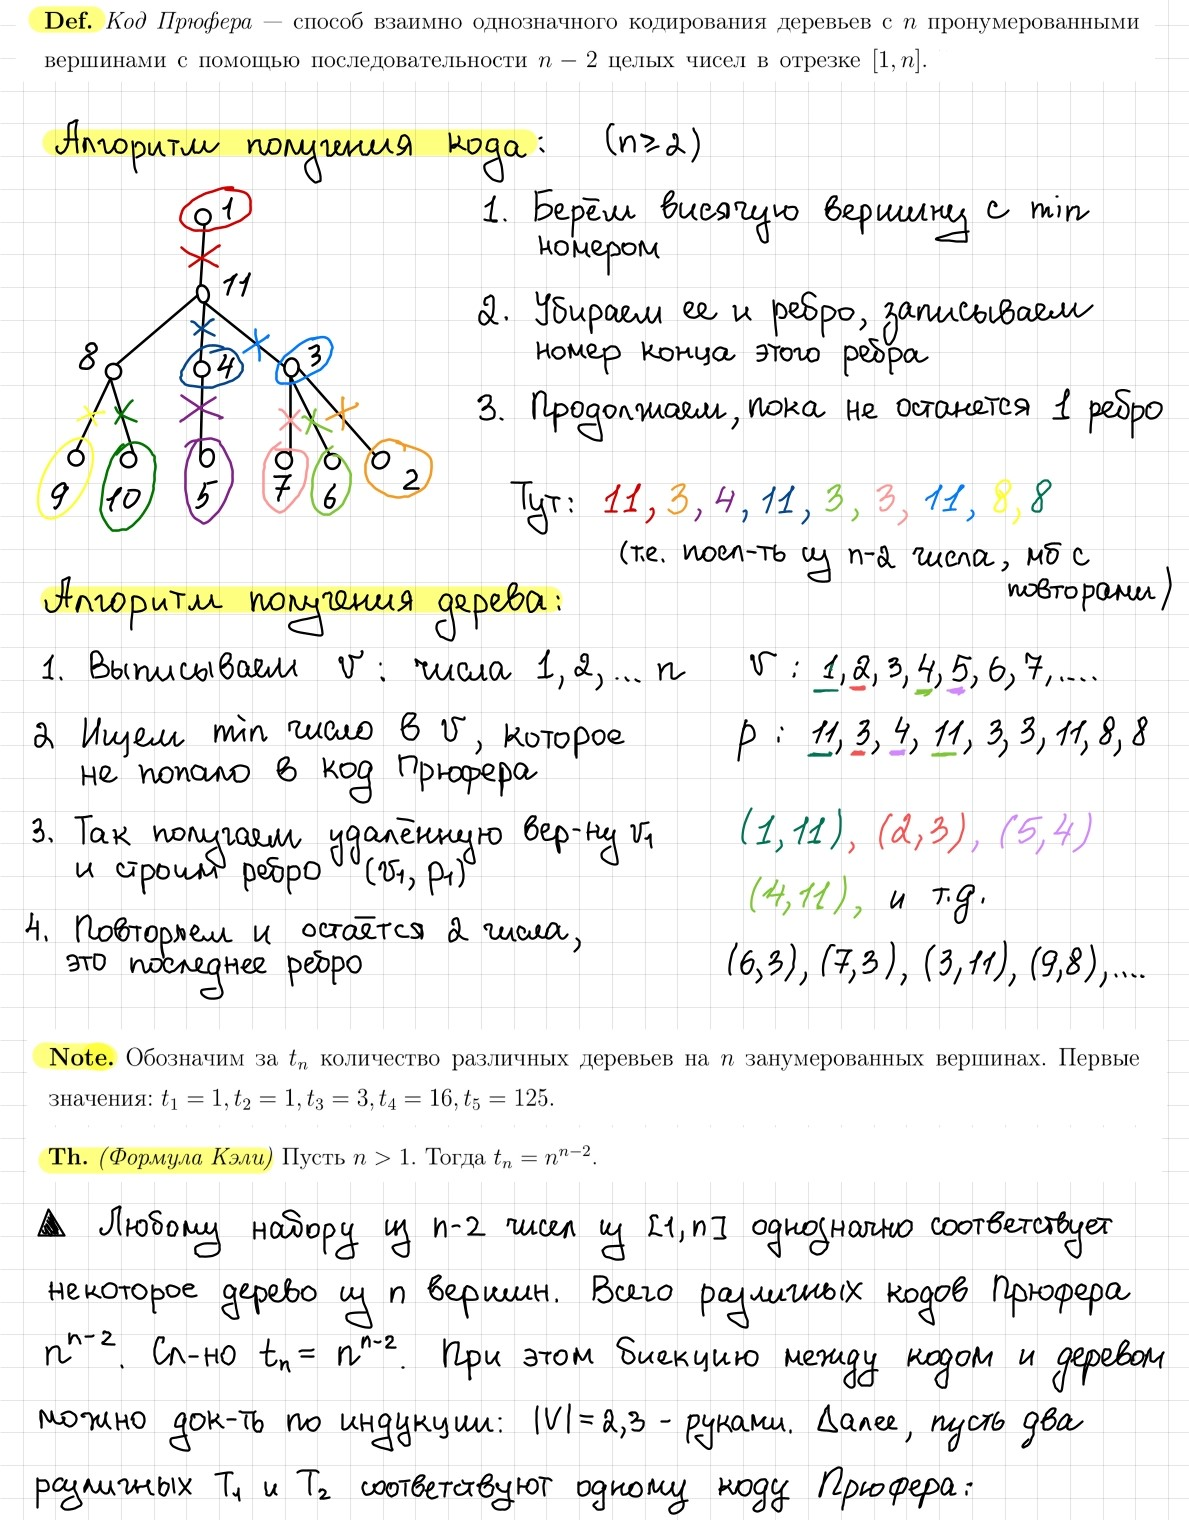
\includegraphics[width=1\linewidth]{sections/Polina/imgs/13.jpg}
\newpage 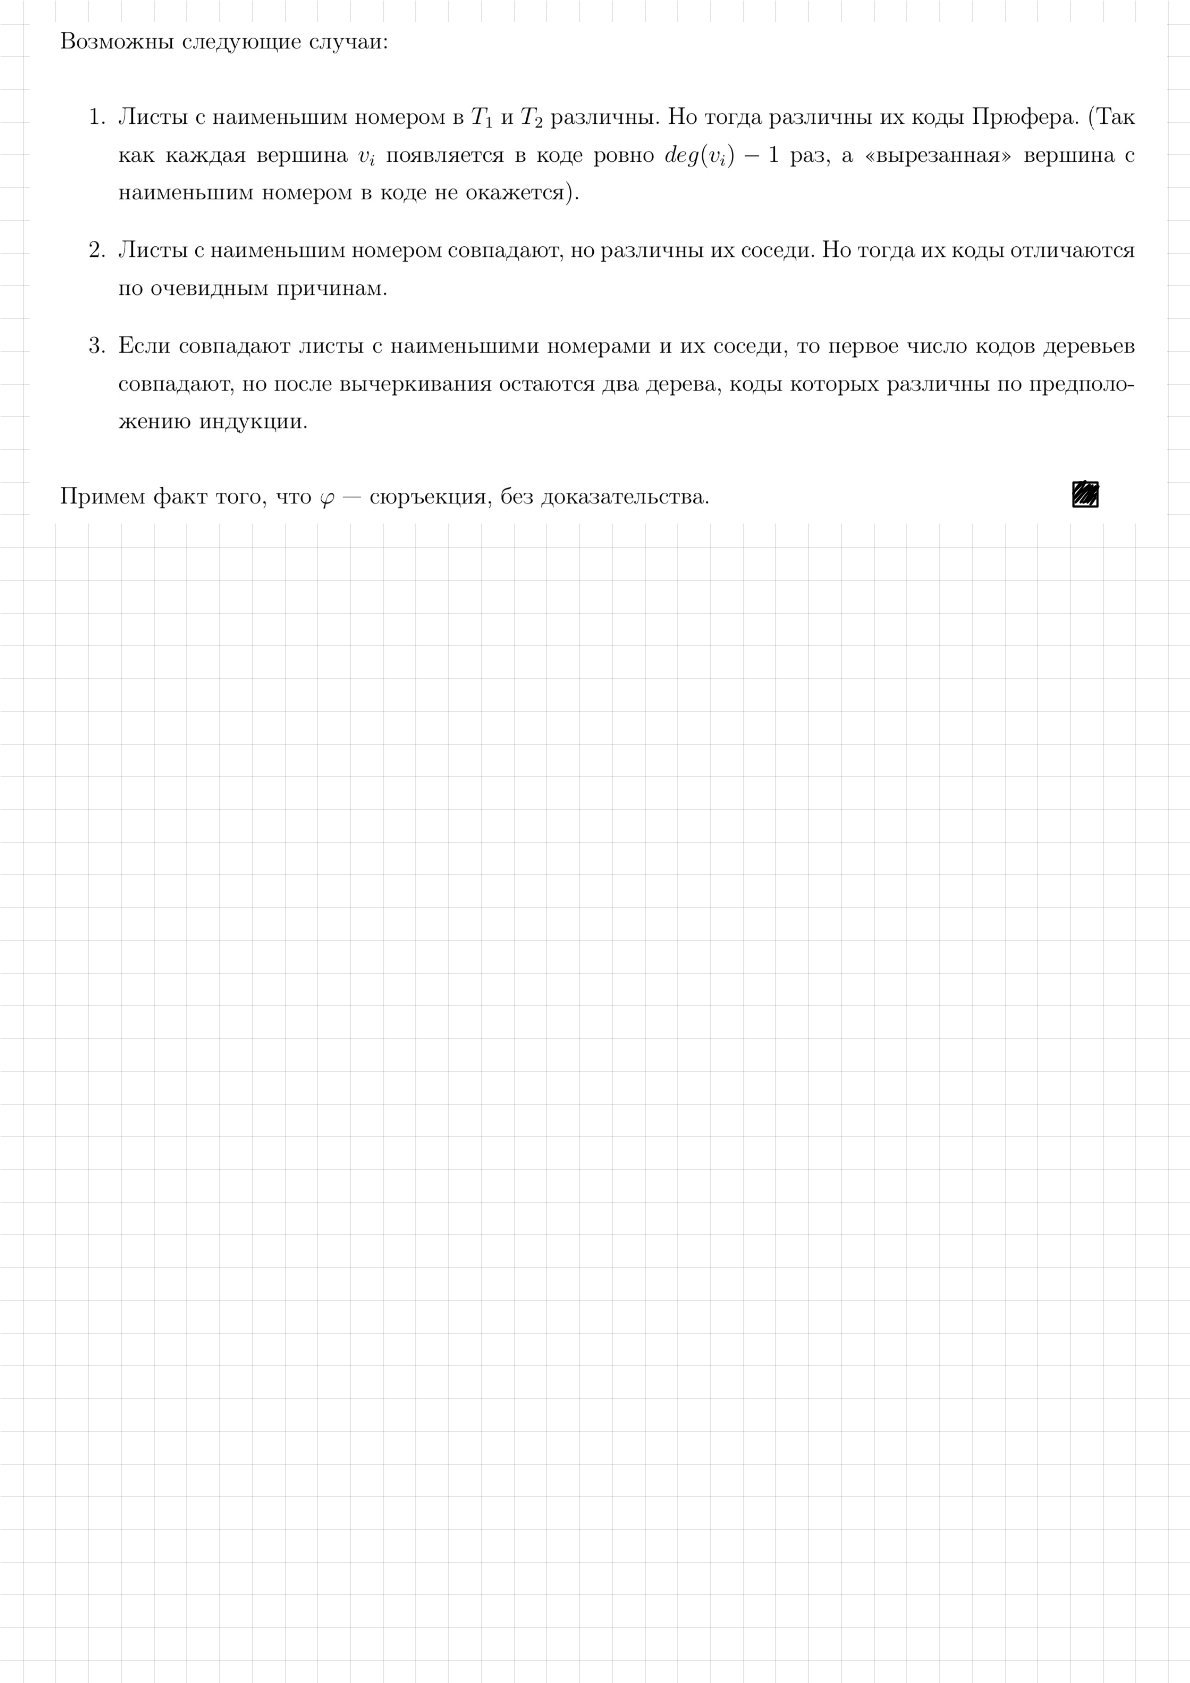
\includegraphics[width=1\linewidth]{sections/Polina/imgs/14.jpg}
\newpage{}

\section{(7) Точная ф-ла для числа унициклических графов. Асимптотика (б/д).}
\textbf{Унициклический граф} - связный граф из n вершин и n рёбер.

Идея: ровно один цикл, т.к. к дереву без циклов добавили ещё одно ребро.

Количество унициклических графов на n вершинах: $u_n$

\Th $u_n = \sum_{k=3}^n C_n^k \frac{(k-1)!}{2} kn^{n-k-1}$

\Proof
Длина цикла в уницикл. графе равна k. $k \in [3; n]$, т.к. нет ни петель, ни кратных рёбер, тогда: 

$C_n^k$ - количество способов выбрать вершины цикла; 

$\frac{(k-1)!}{2}$ - количество способов зафиксировать цикл после того, как вершины выбраны;  

$F_{n, k}$ - количество лесов, в котором k деревьев, причём вершина $i$ принадлежит $i$-ому дереву; $F_{n, k} = kn^{n-k-1}$ (док-во внизу).
\EndProof

\leftbar

Доказательство формулы $F_{n, k}$ с семинара: Нетрудно построить взаимно-однозначное соответствие между корневыми лесами на $n$ вершинах с $k$ деревьями и деревьями на вершинах ${1, 2, \dots, n+1}$, где вершина $n+1$ имеет степень $k$. Из прошлой задачи мы знаем, что таких деревьев $C_{n-1}^{k-1}n^{n-k}$ (выбираем $k-1$ позиций в коде Прюфера для вершины $n+1$, остальное заполняем произвольно). В задаче нас просят посчитать не просто количество корневых лесов на $n$ вершинах с $k$ деревьями, а количество таких лесов, где корнем $i$-го дерева является вершина $i$. В силу симметрии. Каждое k-элементное подмножество множества ${1, 2, \dots, n+1}$ является множеством корней для одинакового числа лесов, поэтому чтобы получить ответ надо поделить количество корневых лесов на $C_n^k$. Таким образом, ответом будем $kn^{n-k-1}$.
\endleftbar

Следствие: $u_n \sim \sqrt{\frac{\pi}{8}} n^{n - \frac{1}{2}}$ - Асимптотика (б/д).
\newpage{}

\section{(9) Асимптотика числа унициклических графов.}
\subsection{4. Регулярные выражения. Теорема Клини о совпадении классов регулярных и автоматных языков. Регулярный автомат, алгоритм построения.}

\Vars \\
Regex (регулярное выражение) обозначим за $R$, \newline Language (язык) -- за $L$, \newline $L(R_i)$ (язык, который задается регулярным выражением $R$) -- $L_i$.

\Def Рекурсивное определение регулярного выражения.

% \begin{minipage}[r]{0.1\linewidth} 
% %\begin{flushright}
%     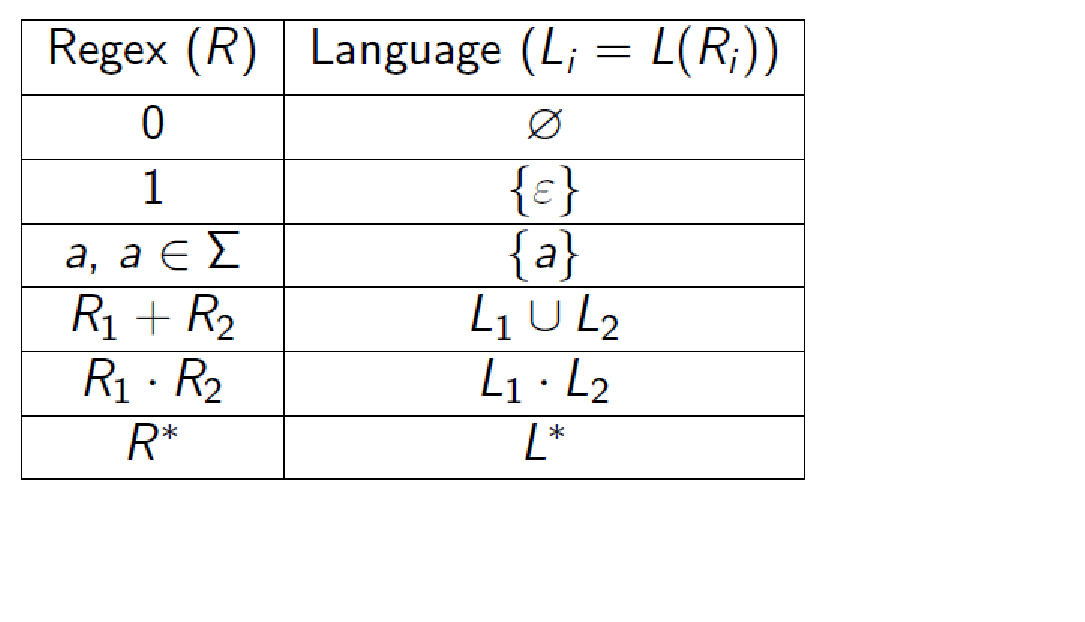
\includegraphics[width=5\linewidth]{images/1_4_1.png}
% %\end{flushright} 
% \end{minipage} 
\begin{center}
    \begin{tabular}{|c|c|}
        \hline
        $Regex (R)$ & $Language (L_i = L(R_i))$ \\
        \hline
        $0$ & $\varnothing$ \\
        $1$ & $\{ \varepsilon \}$ \\
        $a$, $a \in \Sigma$ & $\{ a \}$ \\
        $R_1 + R_2$ & $L_1 \cup L_2$ \\
        $R_1 \cdot R_2$ & $L_1 \cdot L_2$ \\
        $R^*$ & $L^*$ \\
        \hline
    \end{tabular}
\end{center}

Здесь $\varepsilon$ -- пустое слово, <<$\cdot$>> -- операция конкатенации языков (в полученном языке $L_1 \cdot L_2$ лежат слова вида $a_1a_2$, где слово $a_1$ лежит в языке $L_1$, а слово $a_2$ лежит в языке $L_2$), <<$*$>> -- звезда Клини.

Напомним определение звезды Клини: $V^* = \bigcup_{i=0}^{\infty} V^i$ 

\textbf{Приоритет операций} в регулярных выражениях (левее — приоритетнее): $* \rightarrow \cdot \rightarrow +$

\Def Язык $L$ -- регулярный, если он задается регулярным выражением.

\hspace{4ex}

\textbf{Теорема Клини:} Классы регулярных и автоматных языков совпадают.

\Proof Докажем два вложения:

\textbf{1. Регулярные $\subseteq$ Автоматные}

% \begin{figure}[h]
%     \begin{minipage}[h]{0.6\linewidth}
%     Индукция по построению выражения. 
    
%     Немного изменим утверждение -- докажем, что по регулярному выражению можно построить НКА с $1$ завершающим состоянием, который задает тот же язык.\\
    
%     \textit{База}: Построим автоматы для регулярных выражений: 0, 1, a.
%     \end{minipage}
%     \hspace{-4ex} \begin{minipage}[h]{0.5\linewidth}
%     \center{\includegraphics[width=0.6\linewidth]{images/4_base.jpg}}
%     \end{minipage}
% \end{figure}
% Регулярное выражение <<$0$>> -- автомат без завершающих состояний.

% Регулярное выражение <<$1$>> -- в автомате, состоящем из одной вершины, стартовая вершина помечается завершающим состоянием.

% Регулярное выражение <<$a$>> -- в автомате две вершины. Вершина номер $0$ стартовая, вершину номер $1$ помечаем как терминальную. Проводим ребро из $0$ в $1$, на котором пишем букву a.

Индукция по построению выражения. Немного изменим утверждение -- докажем, что по регулярному выражению можно построить НКА с $1$ завершающим состоянием, который задает тот же язык.

\textit{База}: Построим автоматы для регулярных выражений: $0, 1, a \in \Sigma$.
% %картинка%
\begin{figure}[h!]
    \centering
    \includegraphics[scale=0.27]{4_base.jpg}
\end{figure}
% \newline \center{\includegraphics[width=0.29\linewidth]{4_base.jpg}}
% \begin{minipage}[r]{1\linewidth} 
% %\begin{flushright}
%     % 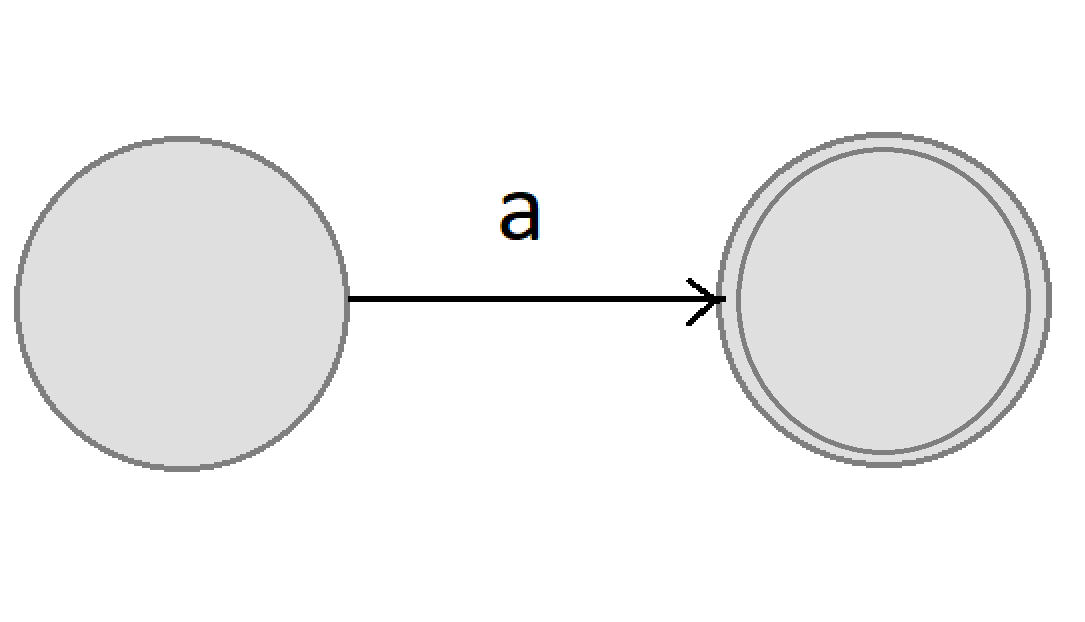
\includegraphics[width=2\linewidth]{images/1_4_2.png}
%     \center{\includegraphics[width=1\linewidth]{images/4_base.jpg}}
% %\end{flushright} 
% \end{minipage} 

\textit{Переход:}

1) $R = R_1 + R_2$. Построим автомат $A_1$ для $R_1$, для которого вершина $S_1$ -- стартовая, а вершина $F_1$ -- единственная терминальная. Для $R_2$ это будут автомат $A_2$ со стартовой вершиной $S_2$ и терминальной $F_2$.
Создадим новую вершину $S$, которая и будет стартовой в новом автомате. Из нее проведем два ребра с $\varepsilon$-переходами в $S_1$ и в $S_2$. Аналогично соединим завершающие в автоматах с новой завершающей вершиной $F$. Нетрудно доказать, что такой автомат задаст тот же язык, что и наше регулярное выражение.

2) $R = R_1 \cdot R_2$. Аналогично прошлому пункту получим автоматы для $R_1$ и $R_2$ с теми же обозначениями. Вершина $S_1$ будет стартовой в нашем новом автомате. Добавим также $\varepsilon$-переход из $F_1$ в $S_2$, уберем терминальность $F_1$.

3) $R = R_1^*$. Построим автомат $A_1$ для $R_1$ со стартовой вершиной $S_1$ и терминальной вершиной $F_1$. Создадим вершину $S$ -- новую стартовую вершину, пометим ее терминальной. Добавим из нее и из $F_1$ $\varepsilon$-переход в $S_1$.

\textbf{2. Автоматные $\subseteq$ Регулярные}

\Note{Регулярный автомат -- НКА, в котором на ребрах записаны регулярные выражения. Докажем утверждение для регулярных автоматов.}

\Note{Всякий НКА задается регулярным автоматом с 1 завершающим состоянием.}

Индукция по $|Q|$ (количеству состояний -- вершин) в регулярном автомате.

\textit{База:}

1) $|Q| = 1$. Тогда в регулярном автомате стартовое состояние является завершающим, и можно однозначно построить регулярное выражение. Такому автомату соответсвует регулярное выражение $a^*$
\newline
\begin{minipage}[r]{0.1\linewidth} 
%\begin{flushright}
    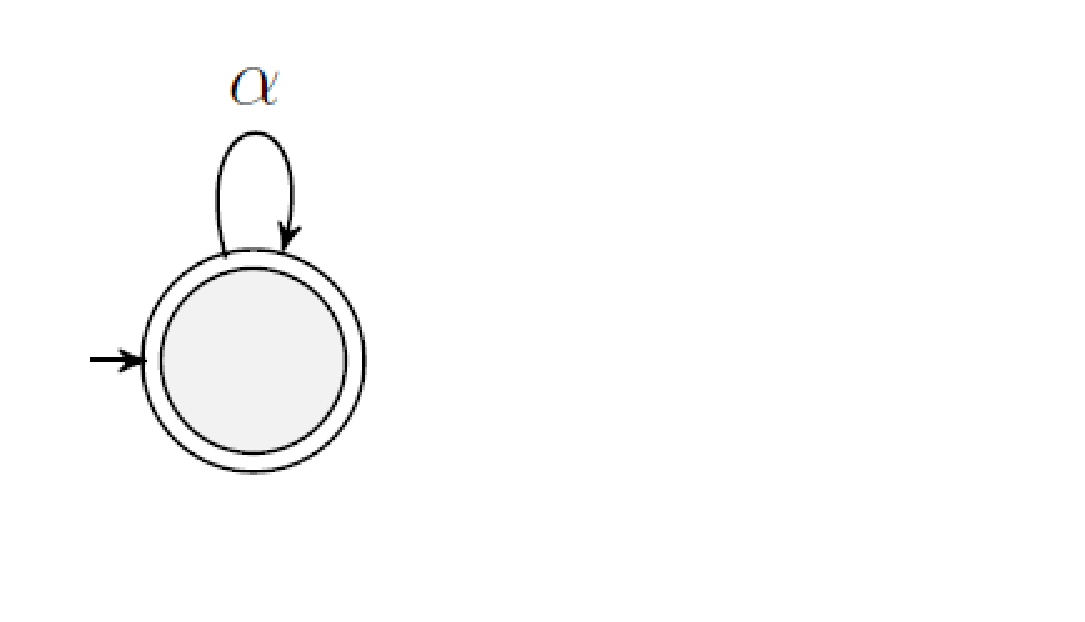
\includegraphics[width=4\linewidth]{images/1_4_3.png}
%\end{flushright} 
\end{minipage} 

2) $|Q| = 2$. Cтартовое состояние и завершающее состояние различны, и можно тоже однозначно построить регулярное выражение. Такому автомату соответсвует регулярное выражение $\alpha^*\beta(\gamma + \delta \alpha^* \beta)^*$
\newline
\begin{minipage}[r]{0.1\linewidth} 
%\begin{flushright}
    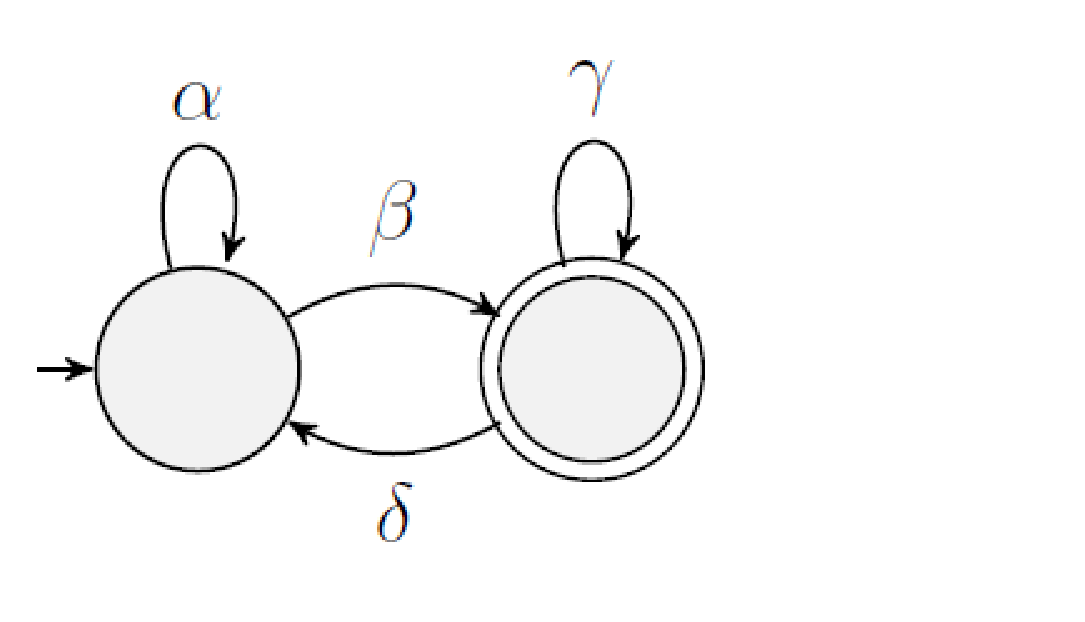
\includegraphics[width=4\linewidth]{images/1_4_4.png}
%\end{flushright} 
\end{minipage} 

Для случая, когда завершающее состояние -- это начальная вершина, регулярное выражение будет $(\gamma + \delta \alpha^* \beta)^*$.

\textit{Переход:}
\Note{Есть нестартовая и незавершающая вершина!}

1) Удаляем кратные ребра:
\begin{minipage}[r]{0.2\linewidth} 
%\begin{flushright}
    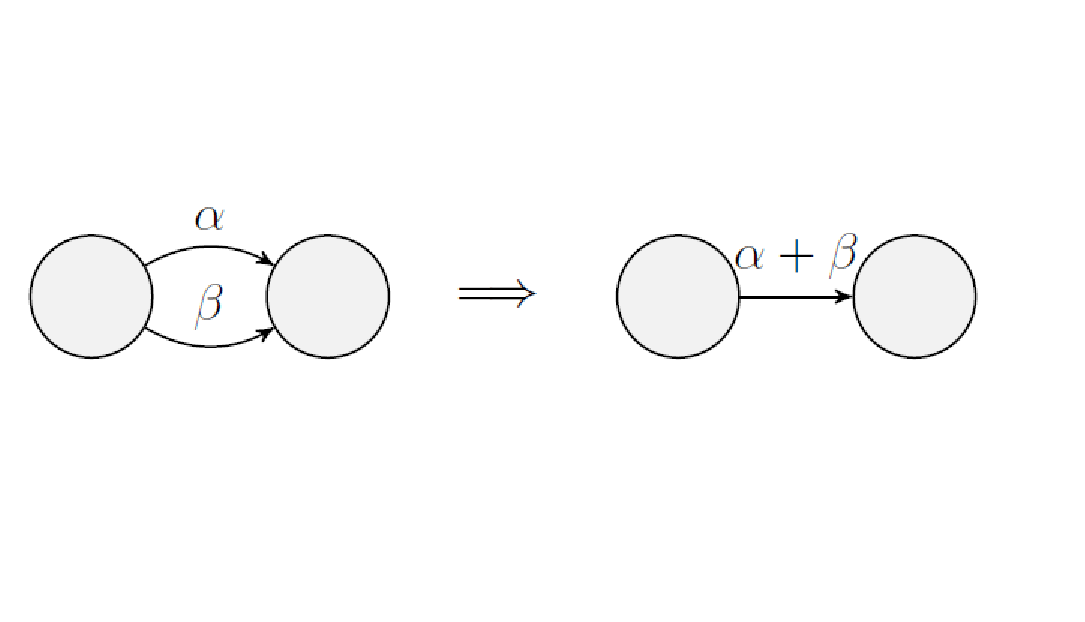
\includegraphics[width=2.5\linewidth]{images/1_4_5.png}
%\end{flushright} 
\end{minipage} 

Кратные ребра означают, что мы можем выбрать, какой символ будем использовать. Именно этот смысл и несет в себе операция <<$+$>>.

2) Добавляем циклы на себя:
\begin{minipage}[r]{0.1\linewidth} 
%\begin{flushright}
    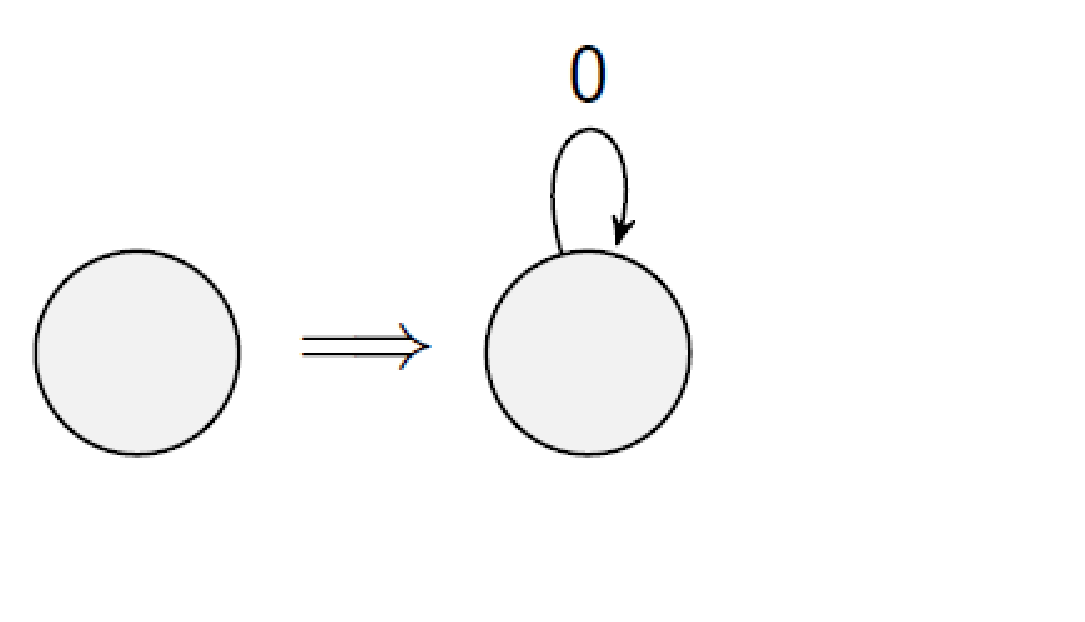
\includegraphics[width=3.5\linewidth]{images/1_4_6.png}
%\end{flushright} 
\end{minipage} 

3) Удаляем нестартовое и незавершающее состояние:

\begin{minipage}[r]{0.1\linewidth} 
%\begin{flushright}
    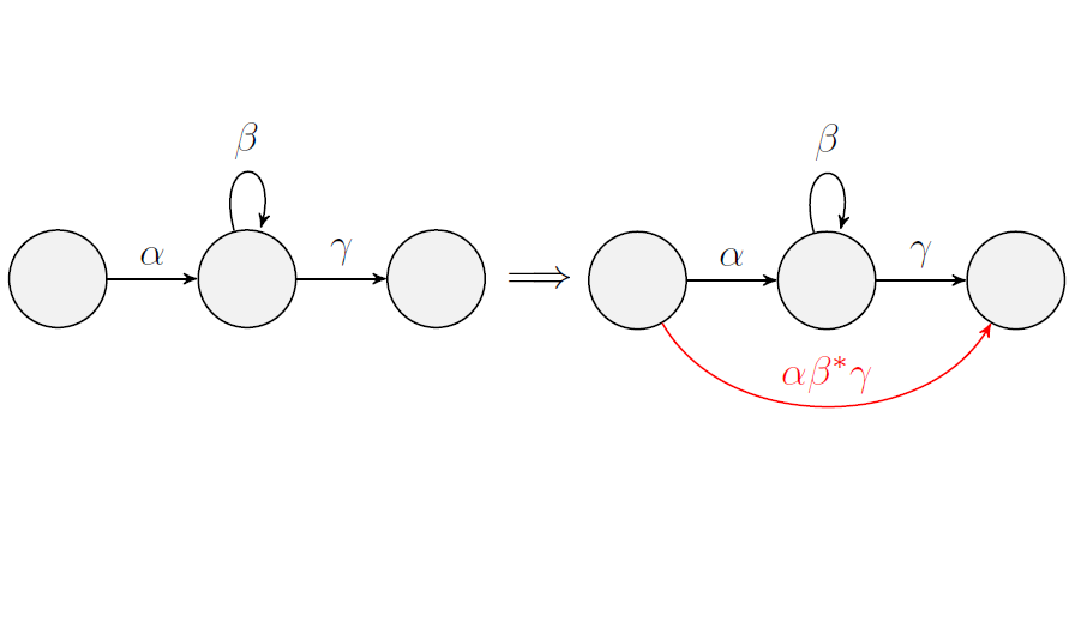
\includegraphics[width=5.5\linewidth]{images/1_4_7.png}
%\end{flushright} 
\end{minipage} 
\newline Теперь у нас на одно сотояние стало меньше, т.е. мы можем воспользоваться утверждением индукции.
\EndProof
\newpage{}

\section{(5) Определение плоских и планарных графов. Формула Эйлера (б/д). Примеры непланарных графов. Критерий Понтрягина–Куратовского планарности графов (б/д).}
\subsection{3. Свойства класса автоматных языков. Замкнутость относительно булевых операций.}

\Def Полный ДКА.
Полный ДКА (ПДКА) - ДКА, для которого выполнено:
$$\forall a \in \Sigma, q \in Q \,\,\, |\Delta (q, a)| = 1$$

\Statement Для любого автоматного языка $L$ существует ПДКА $M$, такой что $L(M) = M$ (т.е. автоматы распознают одинаковое множество слов);

Метод построения ПДКА из ДКА:\\
1) строим ''стоковую'' вершину.\\
2) Добавляем из всех вершин переходы по недостающим буквам в "сток".

\begin{figure}[h]
    \hspace{-4ex} \begin{minipage}[h]{1\linewidth}
    \center{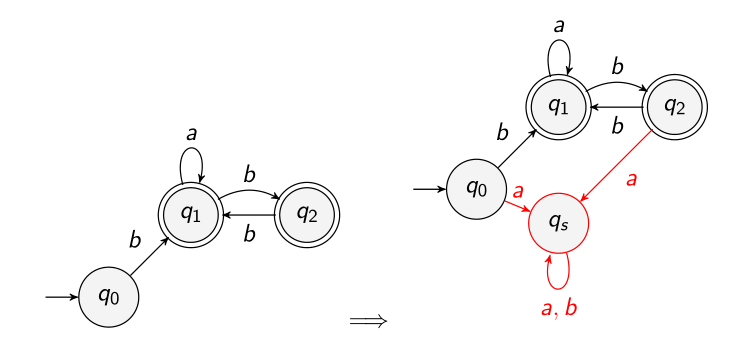
\includegraphics[width=0.6\linewidth]{1_3_1.png}}
    \end{minipage}
    \hspace{-4ex}
\end{figure}

Появятся ли новые слова? - нет, потому что, если мы попали в стоковую вершину, то не сможем ''выбраться'' из неё.

\Def Итерация Клини для языка L.
$$L^* = \cup_{k = 0}^{\infty}L^k$$

\Th Класс автоматных языков замкнут относительно\\
1. Конкатенации\\
2. Объединения\\
3. Пересечения\\
4. Итерации Клини\\
5. Дополнения

\Proof
Далее будем рассматривать только НКА с одним завершающим состоянием.
Для того чтобы после операции у итогового автомата было одно завершающее состояние, добавляем состояние и соединяем завершающие состояния с ним с помощью $\varepsilon$-переходов. (делаем новое состояние - завершающим, а старые - не завершающими)

1) Конкатенация $M_1$ и $M_2$:

Соединяем $\varepsilon$-переходами завершающее состояние $M_1$ со стартовыми состояниями $M_2$.
\begin{center}
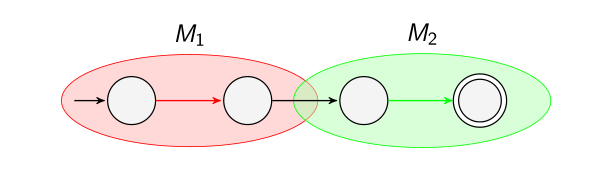
\includegraphics[width=0.45\linewidth]{1_3_2.png}
\end{center}

2) Объединение $M_1$ и $M_2$:

Добавляем стартовое состояние. Соединяем её со стартовыми состояниями $M_1$ и $M_2$ с помощью $\varepsilon$-переходов. 
\begin{center}
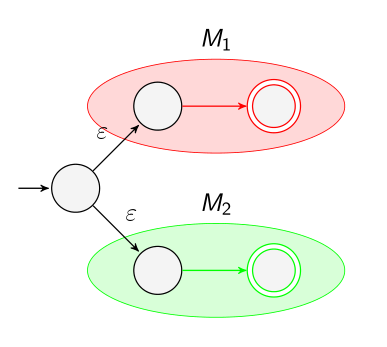
\includegraphics[width=0.25\linewidth]{1_3_3.png}
\end{center}

4) Итерации Клини над $M_1$:

Добавляем стартово-завершающее состояние. С помощью $\varepsilon$-переходов соединяем её с начальными состояниями $M_1$, а завершающее состояния $M_1$ с ней.
\begin{center}
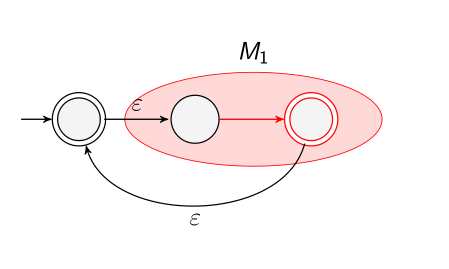
\includegraphics[width=0.32\linewidth]{1_3_4.png}
\end{center}

3) Пересечение $M_1$, $M_2$:

Строим "декартово произведение" автоматов с одно буквенными переходами.

\begin{center}
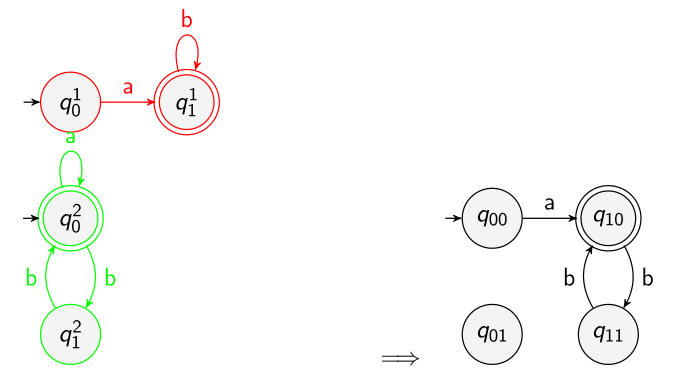
\includegraphics[width=0.55\linewidth]{1_3_5.png}
\end{center}

То есть пересечение будет состоять из состояний, каждому из которых соответствует пара чисел $(i, j)$, это номера состояний из $M_1$ и $M_2$ соответственно, которым это состояние соответствует. И между состояниями $(i_1, j_1)$ и $(i_2, j_2)$ будет проходить ребро с символом $k$, если между $i_1$ и $i_2$ проходило ребро с символом $k$ в $M_1$ и между $j_1$ и $j_2$ проходило ребро с символом $k$ в $M_2$. $(i, j)$ - стартовое состояние, если $i$ - стартовое в $M_1$, $j$ - стартовое в $M_2$. Аналогично с завершающем состоянием. 

5) Дополнение: строим ПДКА и инвертируем терминальность всех состояний.

\newpage{}

\section{(4) Пути и циклы. Простые пути и циклы. Критерии эйлеровости графа и ориентированного
графа.}
\subsection{4. Регулярные выражения. Теорема Клини о совпадении классов регулярных и автоматных языков. Регулярный автомат, алгоритм построения.}

\Vars \\
Regex (регулярное выражение) обозначим за $R$, \newline Language (язык) -- за $L$, \newline $L(R_i)$ (язык, который задается регулярным выражением $R$) -- $L_i$.

\Def Рекурсивное определение регулярного выражения.

% \begin{minipage}[r]{0.1\linewidth} 
% %\begin{flushright}
%     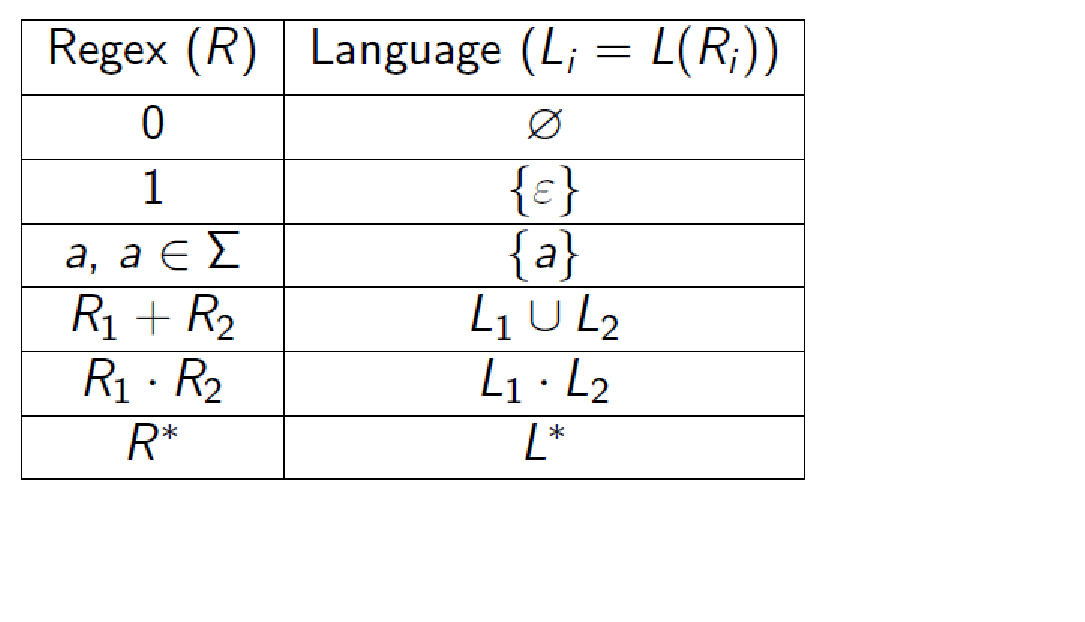
\includegraphics[width=5\linewidth]{images/1_4_1.png}
% %\end{flushright} 
% \end{minipage} 
\begin{center}
    \begin{tabular}{|c|c|}
        \hline
        $Regex (R)$ & $Language (L_i = L(R_i))$ \\
        \hline
        $0$ & $\varnothing$ \\
        $1$ & $\{ \varepsilon \}$ \\
        $a$, $a \in \Sigma$ & $\{ a \}$ \\
        $R_1 + R_2$ & $L_1 \cup L_2$ \\
        $R_1 \cdot R_2$ & $L_1 \cdot L_2$ \\
        $R^*$ & $L^*$ \\
        \hline
    \end{tabular}
\end{center}

Здесь $\varepsilon$ -- пустое слово, <<$\cdot$>> -- операция конкатенации языков (в полученном языке $L_1 \cdot L_2$ лежат слова вида $a_1a_2$, где слово $a_1$ лежит в языке $L_1$, а слово $a_2$ лежит в языке $L_2$), <<$*$>> -- звезда Клини.

Напомним определение звезды Клини: $V^* = \bigcup_{i=0}^{\infty} V^i$ 

\textbf{Приоритет операций} в регулярных выражениях (левее — приоритетнее): $* \rightarrow \cdot \rightarrow +$

\Def Язык $L$ -- регулярный, если он задается регулярным выражением.

\hspace{4ex}

\textbf{Теорема Клини:} Классы регулярных и автоматных языков совпадают.

\Proof Докажем два вложения:

\textbf{1. Регулярные $\subseteq$ Автоматные}

% \begin{figure}[h]
%     \begin{minipage}[h]{0.6\linewidth}
%     Индукция по построению выражения. 
    
%     Немного изменим утверждение -- докажем, что по регулярному выражению можно построить НКА с $1$ завершающим состоянием, который задает тот же язык.\\
    
%     \textit{База}: Построим автоматы для регулярных выражений: 0, 1, a.
%     \end{minipage}
%     \hspace{-4ex} \begin{minipage}[h]{0.5\linewidth}
%     \center{\includegraphics[width=0.6\linewidth]{images/4_base.jpg}}
%     \end{minipage}
% \end{figure}
% Регулярное выражение <<$0$>> -- автомат без завершающих состояний.

% Регулярное выражение <<$1$>> -- в автомате, состоящем из одной вершины, стартовая вершина помечается завершающим состоянием.

% Регулярное выражение <<$a$>> -- в автомате две вершины. Вершина номер $0$ стартовая, вершину номер $1$ помечаем как терминальную. Проводим ребро из $0$ в $1$, на котором пишем букву a.

Индукция по построению выражения. Немного изменим утверждение -- докажем, что по регулярному выражению можно построить НКА с $1$ завершающим состоянием, который задает тот же язык.

\textit{База}: Построим автоматы для регулярных выражений: $0, 1, a \in \Sigma$.
% %картинка%
\begin{figure}[h!]
    \centering
    \includegraphics[scale=0.27]{4_base.jpg}
\end{figure}
% \newline \center{\includegraphics[width=0.29\linewidth]{4_base.jpg}}
% \begin{minipage}[r]{1\linewidth} 
% %\begin{flushright}
%     % 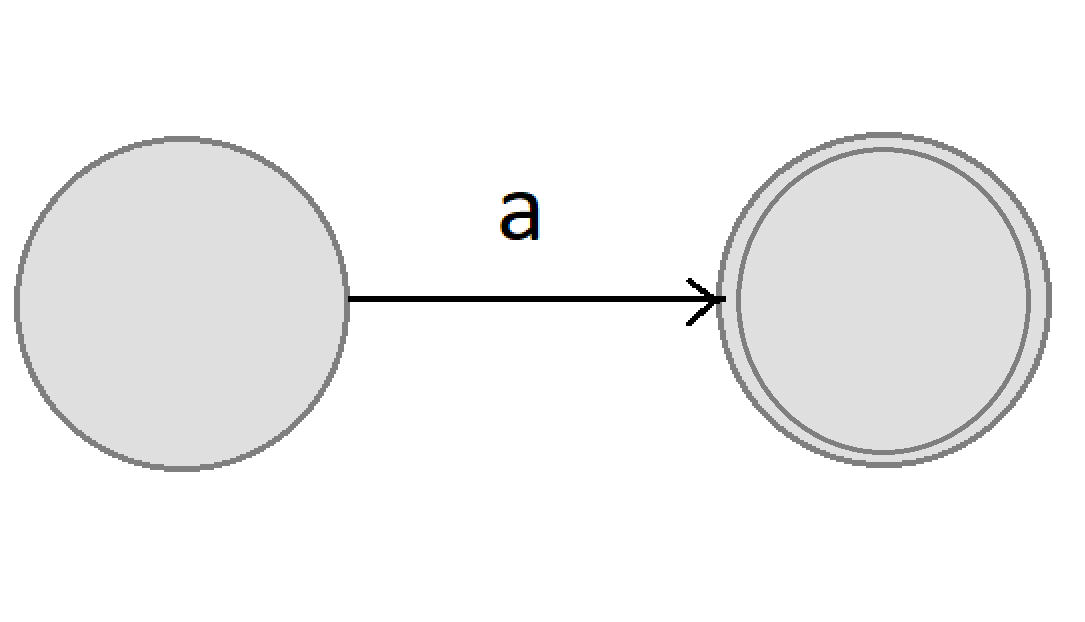
\includegraphics[width=2\linewidth]{images/1_4_2.png}
%     \center{\includegraphics[width=1\linewidth]{images/4_base.jpg}}
% %\end{flushright} 
% \end{minipage} 

\textit{Переход:}

1) $R = R_1 + R_2$. Построим автомат $A_1$ для $R_1$, для которого вершина $S_1$ -- стартовая, а вершина $F_1$ -- единственная терминальная. Для $R_2$ это будут автомат $A_2$ со стартовой вершиной $S_2$ и терминальной $F_2$.
Создадим новую вершину $S$, которая и будет стартовой в новом автомате. Из нее проведем два ребра с $\varepsilon$-переходами в $S_1$ и в $S_2$. Аналогично соединим завершающие в автоматах с новой завершающей вершиной $F$. Нетрудно доказать, что такой автомат задаст тот же язык, что и наше регулярное выражение.

2) $R = R_1 \cdot R_2$. Аналогично прошлому пункту получим автоматы для $R_1$ и $R_2$ с теми же обозначениями. Вершина $S_1$ будет стартовой в нашем новом автомате. Добавим также $\varepsilon$-переход из $F_1$ в $S_2$, уберем терминальность $F_1$.

3) $R = R_1^*$. Построим автомат $A_1$ для $R_1$ со стартовой вершиной $S_1$ и терминальной вершиной $F_1$. Создадим вершину $S$ -- новую стартовую вершину, пометим ее терминальной. Добавим из нее и из $F_1$ $\varepsilon$-переход в $S_1$.

\textbf{2. Автоматные $\subseteq$ Регулярные}

\Note{Регулярный автомат -- НКА, в котором на ребрах записаны регулярные выражения. Докажем утверждение для регулярных автоматов.}

\Note{Всякий НКА задается регулярным автоматом с 1 завершающим состоянием.}

Индукция по $|Q|$ (количеству состояний -- вершин) в регулярном автомате.

\textit{База:}

1) $|Q| = 1$. Тогда в регулярном автомате стартовое состояние является завершающим, и можно однозначно построить регулярное выражение. Такому автомату соответсвует регулярное выражение $a^*$
\newline
\begin{minipage}[r]{0.1\linewidth} 
%\begin{flushright}
    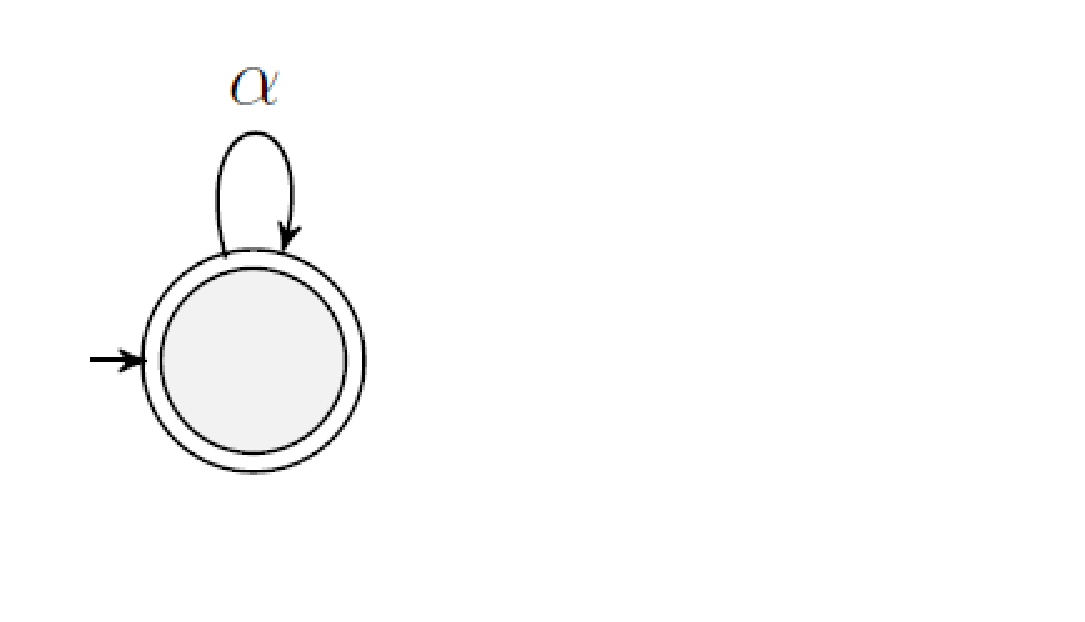
\includegraphics[width=4\linewidth]{images/1_4_3.png}
%\end{flushright} 
\end{minipage} 

2) $|Q| = 2$. Cтартовое состояние и завершающее состояние различны, и можно тоже однозначно построить регулярное выражение. Такому автомату соответсвует регулярное выражение $\alpha^*\beta(\gamma + \delta \alpha^* \beta)^*$
\newline
\begin{minipage}[r]{0.1\linewidth} 
%\begin{flushright}
    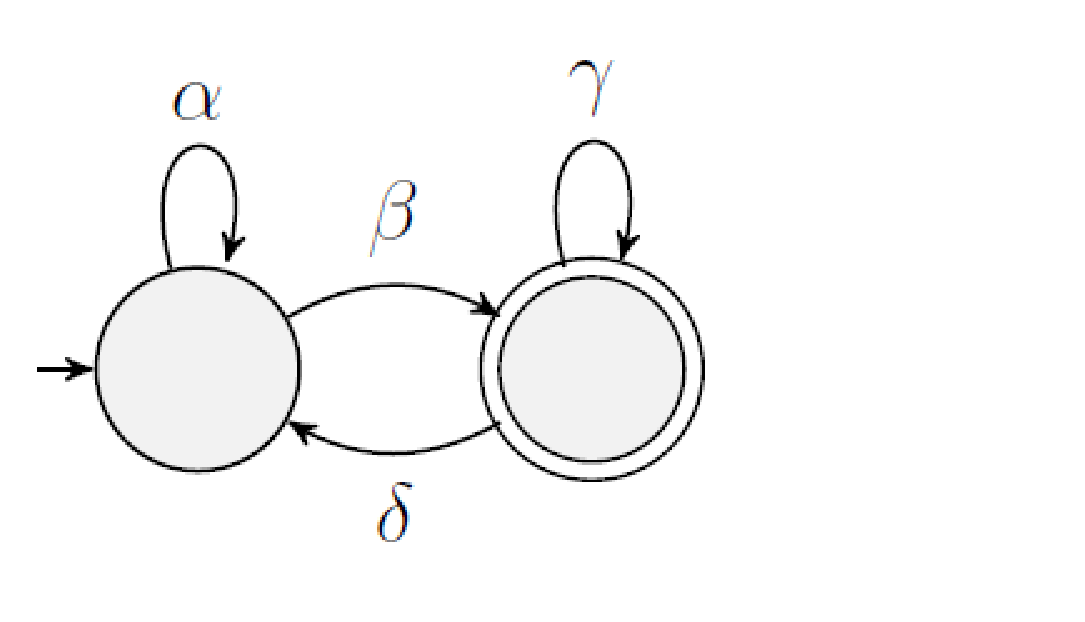
\includegraphics[width=4\linewidth]{images/1_4_4.png}
%\end{flushright} 
\end{minipage} 

Для случая, когда завершающее состояние -- это начальная вершина, регулярное выражение будет $(\gamma + \delta \alpha^* \beta)^*$.

\textit{Переход:}
\Note{Есть нестартовая и незавершающая вершина!}

1) Удаляем кратные ребра:
\begin{minipage}[r]{0.2\linewidth} 
%\begin{flushright}
    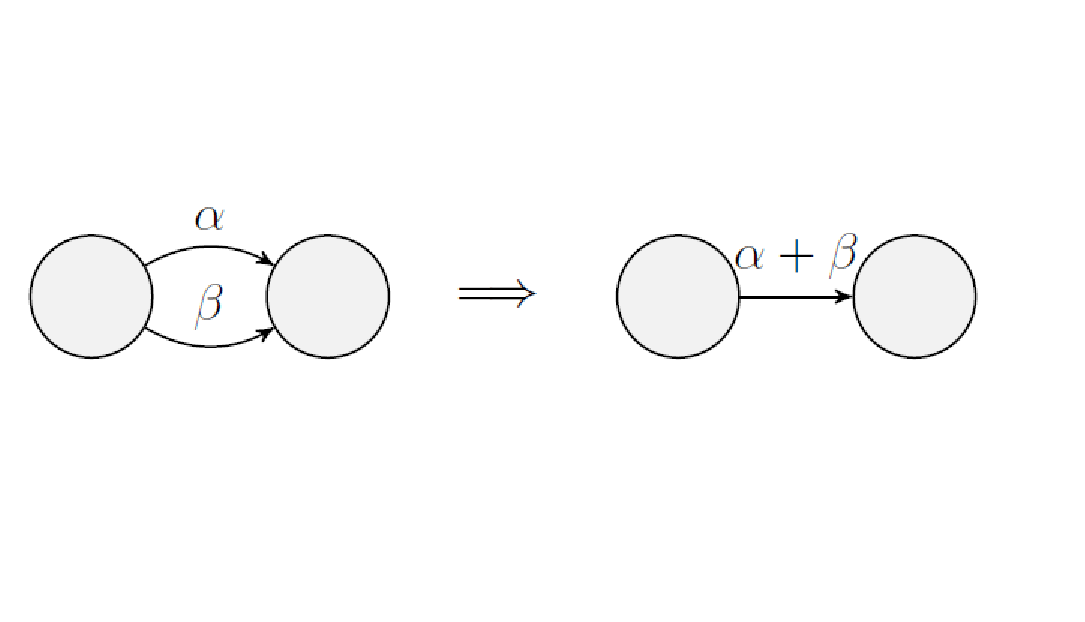
\includegraphics[width=2.5\linewidth]{images/1_4_5.png}
%\end{flushright} 
\end{minipage} 

Кратные ребра означают, что мы можем выбрать, какой символ будем использовать. Именно этот смысл и несет в себе операция <<$+$>>.

2) Добавляем циклы на себя:
\begin{minipage}[r]{0.1\linewidth} 
%\begin{flushright}
    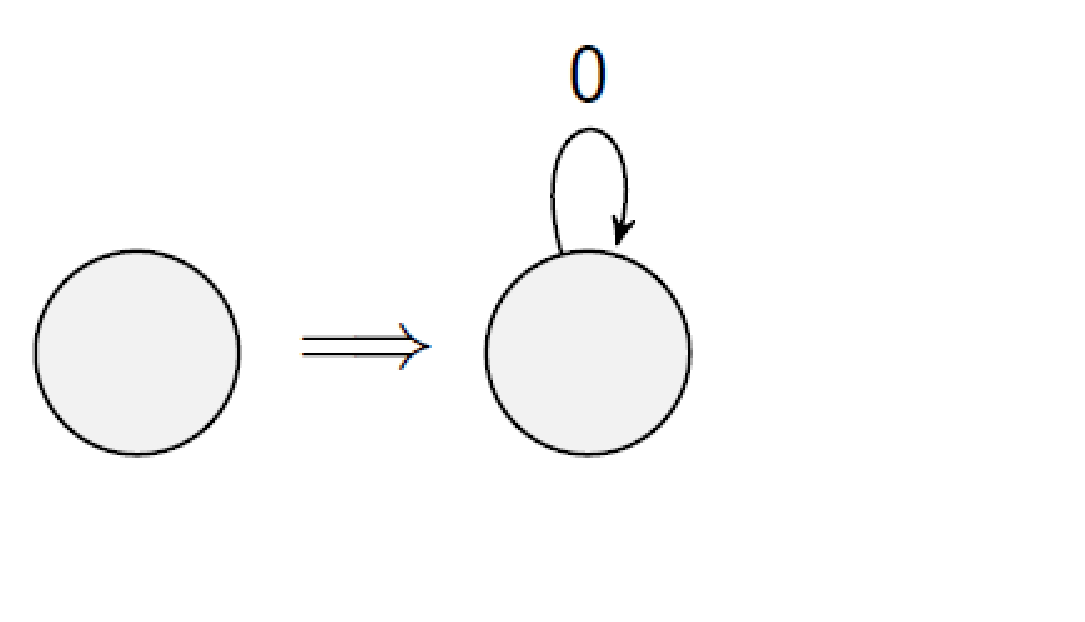
\includegraphics[width=3.5\linewidth]{images/1_4_6.png}
%\end{flushright} 
\end{minipage} 

3) Удаляем нестартовое и незавершающее состояние:

\begin{minipage}[r]{0.1\linewidth} 
%\begin{flushright}
    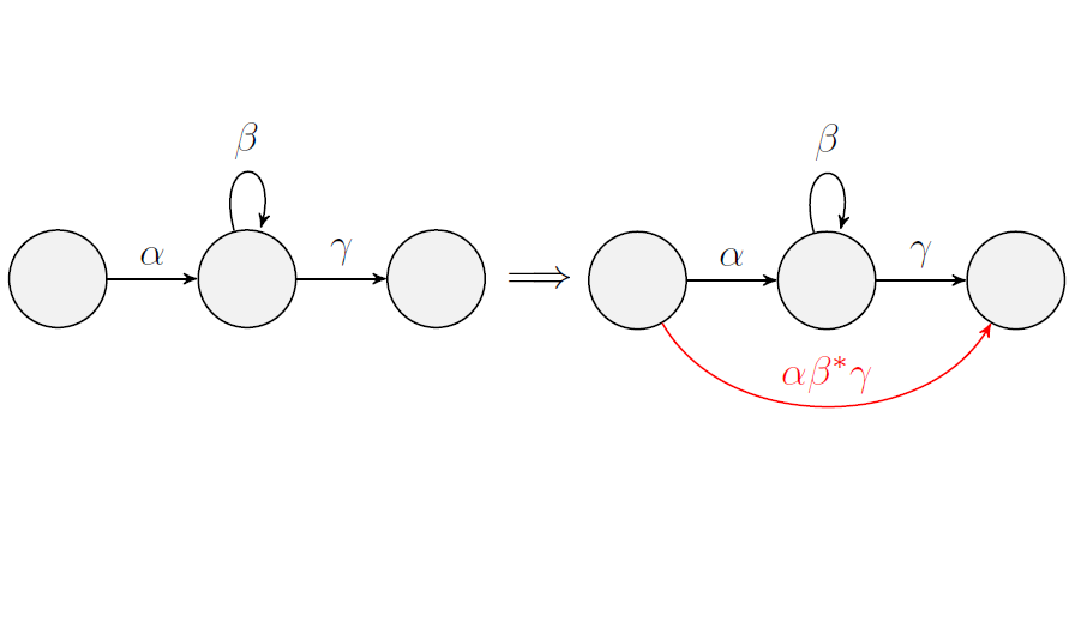
\includegraphics[width=5.5\linewidth]{images/1_4_7.png}
%\end{flushright} 
\end{minipage} 
\newline Теперь у нас на одно сотояние стало меньше, т.е. мы можем воспользоваться утверждением индукции.
\EndProof
\newpage{}

\section{(5) Последовательности и графы де Брёйна. Случай алфавита 0,1 и подслов произвольной длины. Правило 0 лучше 1 (б/д).}
\subsection{5. Минимальный ДКА, его существование.}

\textbf{Мотивировка:} может быть много состояний. А еще не очень понятно, как сравнивать два автомата на эквивалентность. Вернее, если проверять <<в лоб>>, будет долго. Один из способов решить эти проблемы -- минимизация автомата.\\

Пусть $L \subset \Sigma^*$ -- автоматный язык, $M$ -- ПДКА для $L$.

\Def Минимальный ПДКА $M$, распознающий язык $L$, если $M$ -- минимальный по количеству состояний.

\hspace{4ex}

\Def Определим отношение эквивалентности $\sim_L$ на $\Sigma^*:$
$$u \sim_L v \Longleftrightarrow \forall w \in \Sigma^* \,\,(uw \in L \Longleftrightarrow vw \in L)$$

Определение корректно (рефлексивность, симметричность и транзитивность очевидны).

\textit{Множество классов эквивалентности в этом случае:} 
$\Sigma^* /_{\sim_L}:= \{\{u \arrowvert u \sim_L v\} \,\,\arrowvert\,\, v \in \Sigma^*\}$

\Def Определим отношение эквивалентности $\sim_M$ на $Q:$
$$q_1 \sim_M q_2 \Longleftrightarrow \forall w \in \Sigma^*\,\,(\Delta(q_1, w) \in F \Longleftrightarrow \Delta(q_2, w) \in F)$$

Если $q_1 \sim_M q_2$, то состояния можно объединить.

\textit{Напоминание:} Множество вершин, достижимых из $q$ по $w$ -- $\Delta (q, w) = \{ q' | \langle q, w \rangle \vdash \langle q', \varepsilon \rangle \}$..\\

% \hspace{4ex} 
\textbf{Лемма}
Пусть $L_q := \{w \,\arrowvert\, \Delta(q_0, w) = q\}$. Тогда каждый класс эквивалентности в нашем фактор-множестве являетеся объединением классов в $L_q$.

\Proof
Возьмем слово $u \in [u] \in \Sigma^*/_{\sim_L}$, где $[u]$ -- это класс эквивалентности для $u$. Рассмотрим путь по $u$ из $q_0$, а именно,  $q_u = \Delta(q_0, u)$. Для любого слова $w \in [u]$, $q_w = \Delta \brackets{q_0, w}$. Тогда $[u] = \bigcup \limits_{q_w, w \in [u]} L_{q_w}$. Далее докажем, почему это так.
% Из последнего очевидно, что $u \in L_{q_u}$. 

Пусть $v \in [u] \,\Longrightarrow\, v \sim_L u \,\Longrightarrow\, q_v = \Delta \brackets{q_0, v} \,\Longrightarrow\, v \in L_{q_v}$. Тогда $v \in \bigcup \limits_{q_w, w \in [u]} L_{q_w}$.

Пусть $v \in \bigcup \limits_{q_w, w \in [u]} L_{q_w}$. Тогда существует состояние $q_z$, $z \in [u]$, что $v \in L_{q_z} = \{ w | \Delta \brackets{q_0, w} = q_z \}$.
\begin{center}
    $z \in [u] \Longrightarrow z \sim_L u \stackrel{def}{\Longrightarrow} \; \forall w \in \Sigma^* \; \brackets{zw \in L \Longleftrightarrow uw \in L}$
    \begin{equation*}
        \left.
          \begin{array}{ccc}
            v \in L_{q_z} \Longrightarrow & \Delta \brackets{q_0, v} & = q_z \\
            & \Delta \brackets{q_0, z} & = q_z \\
          \end{array}
        \right\} \quad
    \Longrightarrow \quad v \sim_L z \text{ так как $\forall w \in \Sigma^*$ $\Delta \brackets{q_0, vw} \stackrel{(*)}{=} \Delta \brackets{q_0, zw}$}
    \end{equation*}
\end{center}

$\brackets{*}$: $\Delta \brackets{q_0, vw} = \Delta \brackets{\Delta(q_0, v), w} = \Delta \brackets{q_z, w} = \Delta \brackets{\Delta(q_0, z), w} = \Delta \brackets{q_0, zw}$

Так как $v \sim_L z$, $z \in [u]$, то $v \in [u]$. Значит, $[u] = \bigcup \limits_{q_w, w \in [u]} L_{q_w}$, и каждый класс эквивалентности из $\Sigma^* /_{\sim_L}$ — объединение классов в $L_q$. \quad \EndProof

% И так для любого элемента $w \in [u] \hookrightarrow w \in L_{q_w}$. Поэтому \[ [u] \subset \bigcup_{q_w, w \in [u]} L_{q_w}.\]

% Докажем теперь обратное включение. Возьмем $v \in L_{q_w}$. Для него верно $q_v = \Delta(q_0, v) = q_w$. Докажем, что тогда $v \in [w]$ ($[u] = [w]$).

% Возьмем произвольное $m \in \Sigma^*$. Заметим, что тогда верно $vm \in L \Longleftrightarrow wm \in L$, ведь слово $w$ читается из состояния $q_v$ и приводит в завершающее тогда и только тогда, когда то же самое верно и для $q_w$ (просто в силу того, что $q_v = q_w$).


\textbf{Следствие}
$\arrowvert \Sigma^*/_{\sim_L} \arrowvert \leq \arrowvert Q \arrowvert$\\

\textit{Теперь перейдем к минимальному ПДКА, а именно докажем его существование (тут) и единственность с точностью до изоморфизма (билет 6).}\\

\textbf{Лемма} Для любого автоматного языка $L$ существует ПДКА $M'$ такой, что все состояния в $M'$ попарно неэквивалентны.

Что необходимо доказать?\\
1) Переходы и завершающие состояния согласованы\\
2) Распознаваемые языки совпадают\\
3) Состояния попарно неэквивалентны

\Proof Рассмотрим автомат над классами эквивалентности $\sim_M$. Класс эквивалентности $q$ обозначим за $[q]$. $M' = \langle Q /_{\sim_M}, \Sigma, \Delta', [q_0], F' \rangle$, где:

\begin{center}
    $\Delta' = \{ \langle [q_1], a \rangle \rightarrow [q_2] \;|\; \exists \langle q_1, a \rangle \rightarrow q_2 \in \Delta \}$
    
    $F' = \{ [q_f] \;|\; q_f \in F \}$
\end{center}

1) Проверим, что множества $\Delta'$, $F'$ заданы корректно.

Для $\Delta'$: Пусть $q_1 \sim_m q_1'$, и существует $a$ такое, что $\Delta \brackets{q_1, a} \nsim_m \Delta \brackets{q_1', a}$.
\begin{center}
    $q_1 \sim_M q_1' \stackrel{def}{\Longrightarrow} (\forall w \in \Sigma^* \;\;\Delta \brackets{q, w} \in F \Longleftrightarrow \Delta \brackets{q_1', w} \in F)$
    
    $w = au \Longrightarrow (\forall u \in \Sigma^* \;\; \Delta \brackets{q_1, au} \in F \Longleftrightarrow \Delta \brackets{q_1', au} \in F)$
\end{center}

Далее обозначим $\Delta \brackets{q_1, a} = q_2$, a $\Delta \brackets{q_1', a} = q_2'$.
\begin{center}
    $\Delta \brackets{q_1, au} = \Delta \brackets{\Delta(q_1, a), u} = \Delta \brackets{q_2, u}$
    
    $\Delta \brackets{q_1', au} = \Delta \brackets{q_2', u}$
    
    $(\Delta \brackets{q_2, u} \in F \Longleftrightarrow \Delta \brackets{q_2', u} \in F)\; \Longrightarrow q_2 \sim_m q_2'$.
\end{center}

Приходим к противоречию.

Для $F'$:
\begin{center}
    $q_1 \in F$, $q_2 \sim_M q_1 \overset{w = \varepsilon}{\Longrightarrow} (\Delta \brackets{q_1, \varepsilon} \in F \Longleftrightarrow \Delta \brackets{q_2, \varepsilon} \in F)$
    
    Значит, $q_1 \in F \Longleftrightarrow q_2 \in F$
\end{center}

2) Теперь покажем, что $L \brackets{M} = L \brackets{M'}$. 

Для этого нужно показать, что $w \in L \brackets{M} \Longleftrightarrow \Delta \brackets{q_0, w} \in F \stackrel{?}{\Longleftrightarrow} \Delta \brackets{[q_0], w} \in F'$.

Докажем утверждение: $\forall u: \Delta \brackets{q_0, u} = q_1 \Longleftrightarrow \Delta \brackets{[q_0], u} = [q_1]$.

Индукция по длине слова $u$.

\textbf{База.} $|u| = 0 \Longrightarrow u = \varepsilon$. Тогда $\Delta \brackets{q_0, \varepsilon} = q_0$, $\Delta \brackets{[q_0], \varepsilon} = [q_0]$.

\textbf{Переход.} Пусть $u = va$, $v \in \Sigma^*$, $a \in \Sigma$.

\begin{center}
    $\Delta \brackets{q_0, va} = q_1 \Longrightarrow \exists q_2\; \Delta \brackets{q_0, v} = q_2, \;\Delta \brackets{q_2, a} = q_1$
\end{center}

По предположению индукции, $\Delta \brackets{[q_0], u} = [q_2]$, $\Delta \brackets{[q_2], a} = [q_1]$, так как переход $\langle q_2, a \rangle \rightarrow q_1 \in \Delta$ тогда и только тогда, когда $\langle [q_2], a \rangle \rightarrow [q_1] \in \Delta'$. По транзитивности, $\Delta \brackets{[q_0], ua} = [q_1]$.

3) Теперь покажем, что состояния попарно неэквивалентны. В автомате, построенном на классах эквивалентности состояний никакие два состояния не эквивалентны, потому что тогда бы они лежали в одном классе, т.е. были бы одним состоянием.

Пусть $[q_1] \sim_{M'} [q_2]$. Тогда $\forall w : \Delta_{M'} \brackets{[q_1], w} \in F' \Longleftrightarrow \Delta_{M'} \brackets{[q_2], w} \in F'$ по определению. 

\begin{center}
    $[q_{1f}] = \Delta_{M'} \brackets{[q_1], w} \in F'$
    
    $[q_{2f}] = \Delta_{M'} \brackets{[q_2], w} \in F'$
    
    $\exists q_{1f} \in F : \Delta_M \brackets{q_1, w} = q_{1f} \in F \Longleftrightarrow \exists q_{2f} \in F : \Delta_M \brackets{q_2, w} = q_{2f} \in F$
    
    $q_1 \sim_{M} q_2 \Longrightarrow [q_1] = [q_2]$
\end{center}
\begin{flushright}
  \EndProof
\end{flushright} 


\Th $M$ — минимальный ПДКА, распознающий язык $L$, тогда и только тогда, когда любые два состояния попарно неэквивалентны и все состояния достижимы из стартового.

\textit{Теперь запишем более формально:}

\begin{center}
    $M$ — минимальный ПДКА $\Longleftrightarrow \begin{cases} \forall q_1, q_2 \in Q \ q_1 \nsim q_2 \\ \forall q \in Q \ \exists w \in \Sigma^* : \ \langle q_0, w \rangle \vdash \langle q, \varepsilon \rangle \end{cases}$
\end{center}

\Proof

$\Longrightarrow$ Если $q_1 \sim_M q_2$, то $[q_1] = [q_2]$, и их можно объединить в одно состояние, значит, $M$ не был бы минимальным, и тогда из минимальности следует, что $q_1 \nsim_M q_2$. Если среди состояний есть недостижимые, то если их удалить, то множество принимаемых слов не изменится.

$\Longleftarrow$ По следствию из леммы о $L_q$: $|\Sigma^* /_{\sim_L}| \leqslant |Q|$. Рассмотрим $w_1$, $w_2$ такие, что $\Delta \brackets{q_0, w_1} \neq \Delta \brackets{q_0, w_2}$. Введём обозначения:

\begin{center}
    $\Delta \brackets{q_0, w_1} = q_1$
    
    $\Delta \brackets{q_0, w_2} = q_2$
\end{center}

Неэквивалентность состояний $q_1$, $q_2$ означает, что существует слово $w$, что б.о.о:

\begin{center}
    $\Delta \brackets{q_1, w} = \Delta \brackets{q_0, w_1 w} \in F \Longleftrightarrow w_1 w \in L$
    
    $\Delta \brackets{q_2, w} = \Delta \brackets{q_0, w_2 w} \notin F \Longleftrightarrow w_2 w \notin L$
    
    Следовательно, получили что $w_1 \nsim_L w_2$
\end{center}

Тогда для автомата $M$ со множеством состояний $Q'$ выполняется, что $|\Sigma^* /_{\sim_L}| \geqslant |Q'|$, но тогда $|Q| \geqslant |\Sigma^* /_{\sim_L}| \geqslant |Q'|$, и $M$ — минимальный. \quad \EndProof
\newpage{}

\section{(6) Гамильтоновы пути и циклы. Достаточное условие Дирака гамильтоновости графа.}
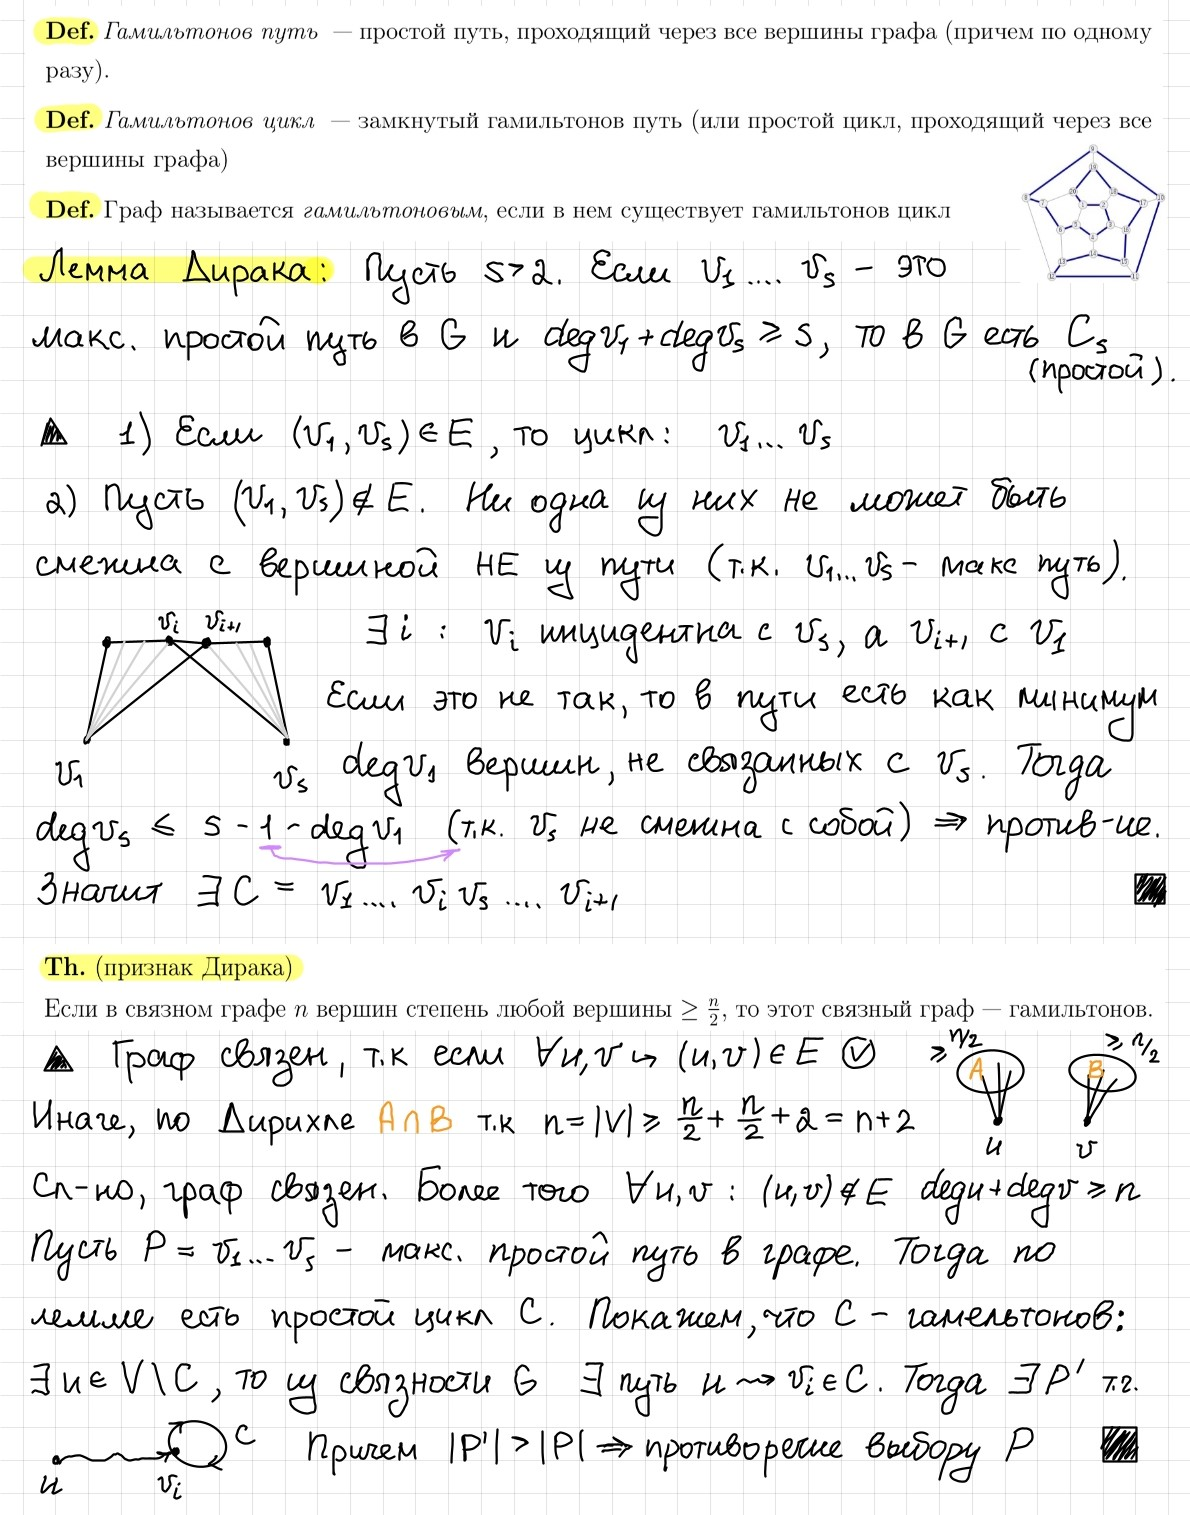
\includegraphics[width=1\linewidth]{sections/Polina/imgs/25.jpg}
\newpage{}

\section{(7) Вершинная связность и число независимости графа. Признак Эрдёша-Хватала (б/д). Гамильтоновость графа 1-пересечений 3-элементных подмножеств n-элементного множества при всех дост. больших n.}
Пусть есть граф $G = (V, E)$, $W \subseteq V$.

\Def W - независимое, если $\forall x, y \in W: (x, y) \notin E$

\Def $\alpha (G) = $ мощность любого самого большого независимого $W$ - число независимости графа.

\Def $\varkappa (G)$ (буква читается каппа) Вершинная связность - min количество вершин, удаление которых приведёт к тому, что граф перестаёт быть связным.

\Th Признак Эрдёша - Хва'тала.

$\alpha (G) \leqslant \varkappa (G)$. Тогда G - гамильтонов.

\Example $V = \{ A \subset \{1, 2, \dots, n \} : |A| = 3\}$. Тогда $|V| = C_n^3 \sim \frac{n^3}{6}$. 

$E = \{ (A, B): |A \cap B| = 1\}$; $\forall A \in V$ $deg A = 3 C_{n-3}^2$ $\Rightarrow$ $|E| = \frac{3 C_{n-3}^2 C_n^3}{2} \sim \frac{n^3}{6} \cdot 3 \cdot \frac{n^2}{4} = \frac{n^5}{8}$

$\alpha(G)$: макс. число "троек", попарные пересечения которых не равны 1, т.е. 0 или 2.

\begin{equation*}
\alpha(G) \geqslant (=) 
 \begin{cases}
   n &\text{$n \equiv 0 (4)$}\\
   n-1 &\text{$n \equiv 1 (4)$} \\
   n-2 &\text{$n \equiv 2, 3 (4)$}
 \end{cases}
\end{equation*}
(Конструкция: разбиваем на четвёрки элементов, внутри каждой четвёрки берём все подмн-ва (они пересекаются по 2 элементам всегда), а разные четвёрки пересекаются по 0).

\Th $\alpha(G) \leqslant n$ для графа в примере.

\Proof Зафиксируем $W = \{ A_1, A_2, \dots, A_t \}$ - независимое подмножество. 

Сопоставим каждому $A_i \rightarrow \overline{x_i} = (x^1, \dots, x^n) \in \Z_2^n, x^j \in \{0, 1\}$, причём 1 стоят на позициях, которые принадлежат множеству $A_i$.

$|A_i \cap A_j| = (\overline{x_i}, \overline{x_j})$. Осталось доказать, что $x_1, \dots, x_t$ ЛНЗ, тогда очевидно, что $|W| = t \leqslant n$, в силу размерности пространства.

Докажем, что $x_1, \dots, x_t$ ЛНЗ в $\Z_2^n$. $c_1x_1 + c_2x_2 + \dots + c_tx_t = \overline{0}$. Домножим обе части равенства на $x_1$, получим: $c_1(x_1, x_1) + c_2 (x_2, x_1) + \dots + c_t (x_t, x_1) = 0$; но все скалярные произведения, кроме $(x_1, x_1)$, равны 0 в $\Z_2$, т.к. они равны либо 0, либо 2, а $(x_1, x_1) \equiv 1 (2)$, значит, $c_1 = 0$. Так можно доказать для любого коэффициента, т.е. это тривиальная линейная комбинация. \EndProof

Оценка на $\varkappa(G)$. Зафиксируем вершины $x, y$, $f(x, y)$ - количество их общих соседок. Тогда $\varkappa(G) \geqslant min_{x, y} f(x, y)$ для любого графа (очевидно). 

Для нашего графа G если $x \cap y = 0$, то $f(x, y) = 3 \cdot 3 \cdot (n - 6)$, т.к. нужно, чтобы из первого множества был один из 3х элементов, из 2-ого один из 3х элементов, а 3й элемент отличен от элементов из этих 2х мн-в.

Если $x \cap y = 1$, то $f(x, y) = C_{n-5}^2 + 2 \cdot 2 \cdot (n - 5)$, первое слагаемое - это если "соседи" содержат элемент, по которому пересечение, второе - не содержат.

Аналогично, если $x \cap y = 2$, то $f(x, y) = 2 \cdot C_{n-4}^2 + n - 4$.

Очевидно, что при больших n минимально $9(n-6) > n \geq \alpha(G)$, значит, такие графы гамильтоновы.
\newpage{}

\section{(7) Вершинная связность и число независимости графа. Признак Эрдёша-Хватала.}
Во всём документе $G=(V, E)$ $-$ зафиксированный граф.

\Def Если $W \subseteq V$ и $\forall x, y \in W((x, y) \notin E)$, то $W$ $-$ \textit{независимое множество}.

\Def \textit{Число независимости графа $G$} $-$ наибольшая мощность независимого множества $G$, обозначается $\alpha(G)$.

\Def множство $W \subseteq V$ \textit{развязывающим}, если $G \Big|_{V \setminus W}$ не связен. \textit{Вершинная связность $G$} $-$ мощность наименьшего развязывающего множества, обозначается $\varkappa(G)$.

\textbf{Теорема(Эрдёша-Хватала):} Если $\alpha(G) \leqslant \varkappa(G)$, то $G$ $-$ гамильтонов.
\begin{wrapfigure}{r}{0.20\linewidth}
				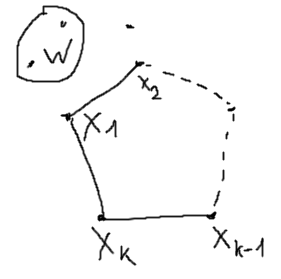
\includegraphics[scale = 0.40]{images/E-H_graph.png}
				\caption{Иллюстрация графа}
\end{wrapfigure} \\
\Proof Предположим противное: в таком графе нет гамильтонового цикла. Тогда рассмотрим любой самый длинный простой цикл $C=\{x_1, ..., x_k\}$. Рассмотрим граф $G'=G \big |_{V \setminus C}$. В $G'$ рассмотрим произвольную компоненту связности $W$. 

\textbf{Множество соседей $W$ в графе $G$} $-$ $N_W(G)= \newline \left \{ y \in V \setminus W : \exists x \in W\left( (x, y) \in E \right) \right \}$.

\underline{Утв. 1}: $N_W(G) \subset C$.

\underline{Утв. 2}: Соседние вершины $C$ не могут принадлежать $N_W(G)$ одновременно (иначе можно удлинить цикл).

\underline{Утв. 3}: $\varkappa(G) \leqslant |N_W(G)|$.

\underline{Утв. 4}: Назовём $M=\{x_{i+1}: x_i \in N_W(G) \}$. По утв. 2 \newline
$M \cap N_W(G) = \varnothing$ и $|M|=|N_W(G)|$. Тогда $M$ $-$ независимое множество вершин. \\
Док-во утв. 4: Предположим противное: в $M$ есть рёбра между вершинами. Тогда выберем в цикле вершины $x_i, x_{i+1}, x_j, x_{j+1}$, при этом между $x_{i+1}$ и $x_{j+1}$ есть ребро.
Тогда можно удлинить цикл: вместо $x_1\!\! \shortrightarrow\!\! x_2\!\! \shortrightarrow\!\! ...\!\! \shortrightarrow\!\! x_i\!\! \shortrightarrow\!\! x_{i+1}\!\! \shortrightarrow\!\! ...\!\! \shortrightarrow\!\! x_j\!\! \shortrightarrow\!\! x_{j+1}\!\! \shortrightarrow\!\! ...\!\! \shortrightarrow\!\! x_k\!\! \shortrightarrow\!\! x_1$ новый цикл $x_1\!\! \shortrightarrow\!\! x_2\!\! \shortrightarrow\!\! ...\!\! \shortrightarrow\!\! x_i\!\! \shortrightarrow\!\! a\!\! \shortrightarrow\!\! ...\!\! \shortrightarrow\!\! b\!\! \shortrightarrow\!\! x_j\!\! \shortrightarrow\!\! ...\!\! \shortrightarrow\!\! x_{i+1}\!\! \shortrightarrow x_{j+1}\!\! \shortrightarrow\!\! ...\!\! \shortrightarrow\!\! x_k\!\! \shortrightarrow\!\! x_1$ ($a, b \in W$). будет как минимум на 1 вершину длиннее, что противоречит предположению, что $C$ - наидлиннейший.

\underline{Утв. 5}: Пусть $x \in W$. Тогда $M \bigcup {x}$ $-$ независимое множество.

Тогда из утв. 5 $\alpha(G) \geqslant |M|+1$, но из утв. 3 $\varkappa(G) \leqslant |M|$. Значит, $\varkappa(G) < \alpha(G)$, что противоречит условию теоремы. \EndProof
\begin{center}
    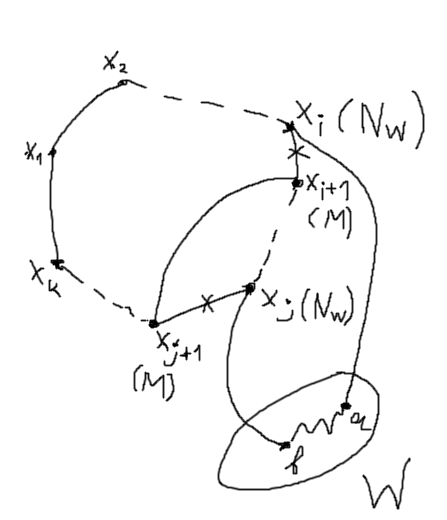
\includegraphics[scale = 0.40]{images/E-H_cycle_lengthening.png}
\end{center}
\newpage{}


\section{(5) Теорема Турана о числе ребер в графе с данным числом вершин и числом независимости.}
\setcounter{section}{6}

\section{Понятия образа и прообраза множества при соответствии. Критерий равенства образа пересечения и пересечения образов. Аналогичные критерии с объединением и разностью.} 
\textbf{Соответствие} между множествами A и B - произвольное подмножество декартова произведения $F \subset A \times B$. Обозначение: $F: A \to B$; иногда, чтобы подчеркнуть, что одному элементу из A может соответствовать несколько элементов из B, пишут: $F:A\rightrightarrows B$. 
\\
\par
Пусть $F: A \to B$ - соответствие, $S \subset A$, $T \subset B$. Тогда \textbf{образ} множества S - множество всех элементов B, соответствующих какому-то элементу S. Формально: $F(S) = \bigcup_{s \in S} F(s) \subset B $. \textbf{Прообраз} множества Т - множество элементов А, которым соответсвует хотя бы один элемент Т. Формально: $F^{-1}(T) = \left\{ a: F(a) \cap T \neq \varnothing \right\}$ 
\\
\par
\emph{ Образ пересечения любых двух множеств равняется пересечению образов тех же множеств $\iff$ соответствие инъективно. } 
\\
$\blacktriangle$
Пусть соответствие не инъективно. Тогда найдутся такие $a_1$ и $a_2$, что $F(a_1)$ и $F(a_2)$ пересекаются. Тогда $F(\left\{a_1\right\} \cap \left\{a_1\right\}) = F(\varnothing) = \varnothing$, но $F(\left\{a_1\right\}) \cap F(\left\{a_2\right\}) = F(a_1) \cap F(a_2)$ не пуст по предположению. Значит, образ пересечения множеств $\left\{ a_1\right\}$ и $\left\{ a_2\right\}$ не равен пересечению образов. \par
Теперь пусть соответствие инъективно. Рассмотрим произвольные подмножества S и Q множества А. Докажем, что $F(S \cap Q) = F(S) \cap F(Q)$. Для этого докажем включение в обе стороны. Вначале пусть $y \in F(S \cap Q)$. Это значит, что $y \in F(x)$ для некоторого $x \in S \cap Q$. Тогда $x \in S$ и $x \in Q$. А раз $y \in F(x)$, то $y \in F(S)$ и $y \in F(Q)$. Значит, $y \in F(S) \cap F(Q)$. (Это включение верно для всех соответствий). \par
Теперь пусть $y \in F(S) \cap F(Q)$. Значит, $y \in F(x_1)$ для некоторого $x_1 \in S$ и $y \in F(x_2)$ для некоторого $x_2 \in Q$. Но при $x_1 \neq x_2$ в силу инъективности множества $F(x_1)$ и $F(x_2)$ не пересекаются. А их пересечение содержит хотя бы y. Значит, $x_1 = x_2 = x$, и $x \in S \cap Q$. А так как $y \in F(x)$, то получаем $y \in F(S \cap Q)$.
$\blacksquare$ \\
\par
\emph{ Образ объединения любых двух множеств равняется объединению образов тех же множеств - выполняется для любых соответствий. } \\
$\blacktriangle$
1) $\left.
  \begin{array}{ccc}
    A \subseteq A \cup B \Rightarrow F(A) \subseteq F(A \cup B) \\
    B \subseteq A \cup B \Rightarrow F(B) \subseteq F(A \cup B) \\
  \end{array}
\right\} \Rightarrow F(A) \cup F(B) \subseteq F(A \cup B) $ \\
2) $y \in F(A \cup B) \Rightarrow \exists x \in A \cup B: y = F(x) \Rightarrow \exists x \in A \cup x \in B: y = F(x) \Rightarrow$ \\
$\Rightarrow y \in F(A) \cup y \in F(B) \Rightarrow y \in F(A) \cup F(B) \Rightarrow  F(A \cup B) \subseteq F(A) \cup F(B) $; \\
Из пунктов 1 и 2 следует, что $F(A \cup B) = F(A) \cup F(B) $
$\blacksquare$ \\
\par
\emph{ Образ разности любых двух множеств равняется разности образов тех же множеств $\iff$ соответствие инъективно. } \\
Доказательство аналогично доказательству для пересечения.
\newpage{}

\section{(4) Соотношения между хроматическим числом, числом независимости и кликовым числом.}
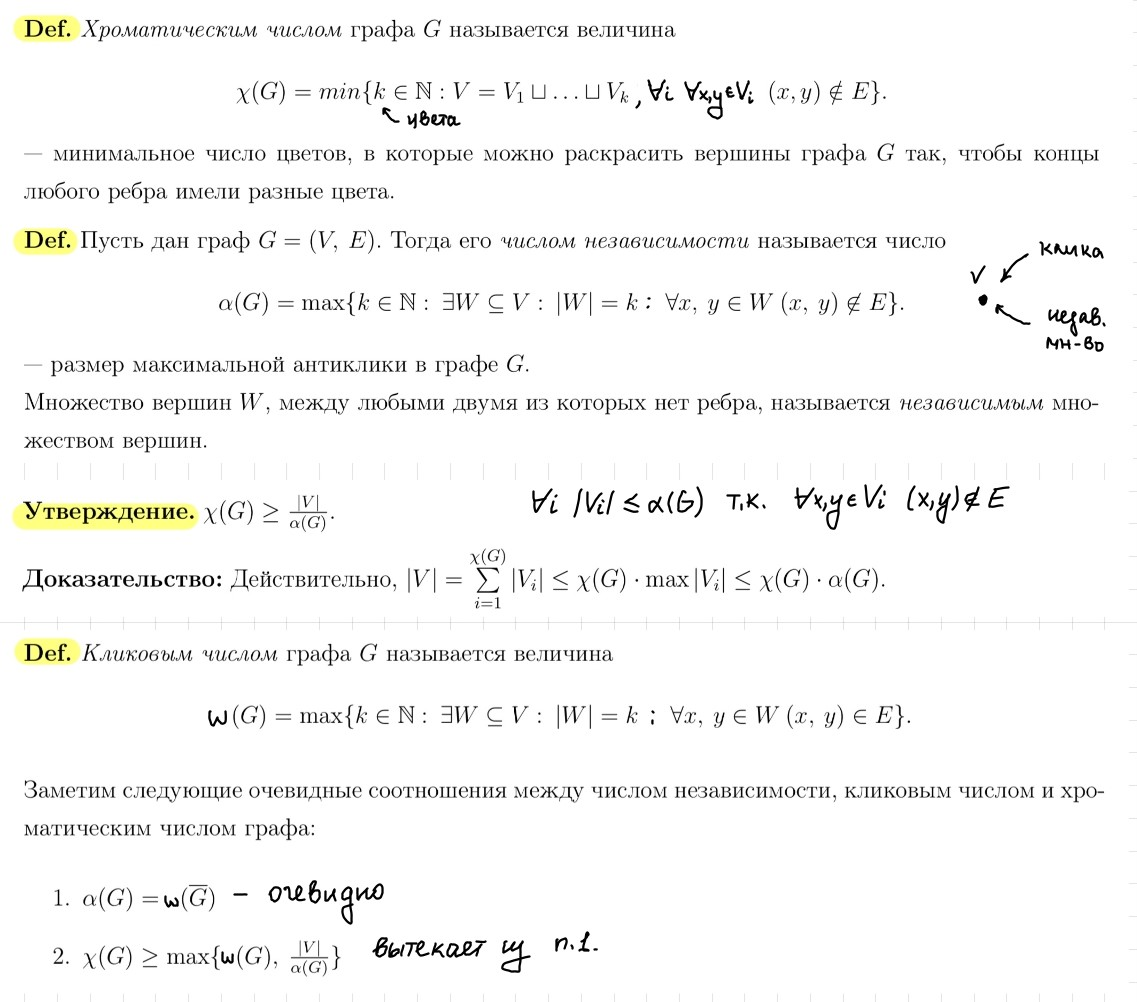
\includegraphics[width=1\linewidth]{sections/Polina/imgs/5.jpg}
\newpage{}

\section{ (4) Числа Рамсея R(s, t): точные значения для s + t $\leq$ 7. Рекуррентная верхняя оценка Эрдёша–
Секереша}
\textbf{Определение} \textit{Число Рамсея R(n,m)}  — наименьшее из таких чисел $x \in N$, что при любой раскраске ребер полного графа на $x$ вершинах в два цвета найдется клика на $n$ вершинах с ребрами цвета 1 или клика на $m$ вершинах с ребрами цвета 2
\\
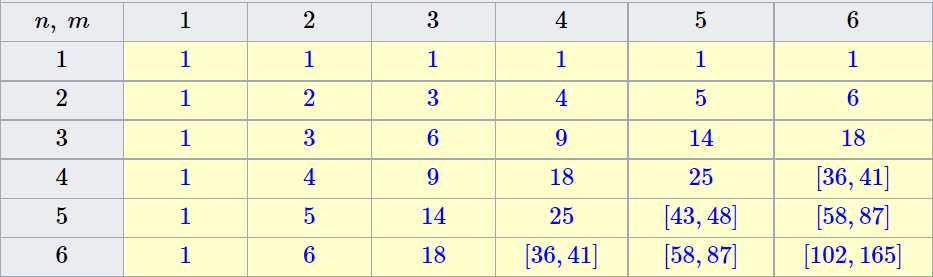
\includegraphics[]{polina_1.PNG}
\begin{itemize}
    \item [1] $R(1,t) = 1$
    \item[2] $R(2,t) = t$
    \item[3] $R(3,3) = 6$ \\
    Возьмем какую-нибудь вершину графа на 6 вершинах. Тогда по приницпу Дирихле из нее выходит либо 3 ребра первого цвета, либо три ребра второго цвета. БОО пусть первого цвета. Тогда рассмотрим треугольник, образованный концами этих ребер. 
    
    Либо у него есть ребро первого цвета, и тогда мы нашли треугольник первого цвета
    
    Либо таких ребер нет, тогда мы нашли треугольник второго цвета.
    
    Пример, почему не можем взять меньше вершин:\\
    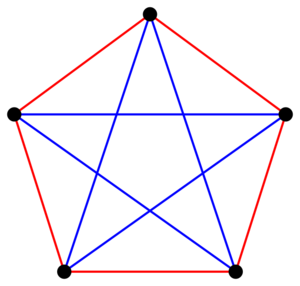
\includegraphics[]{polina_2.png}
    \item[4] То, что $R(4,3) \leq R(3,3)+R(4,2) - 1 = 9$
    Почему 8 вершин нельзя:\\
    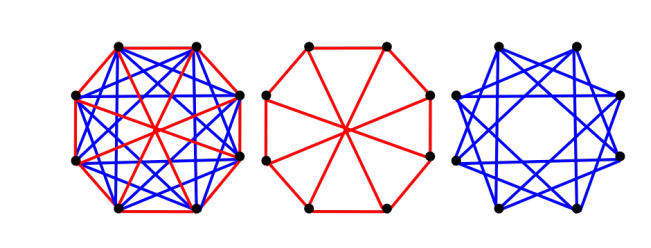
\includegraphics[]{polina_3.PNG}
\end{itemize}
\textbf{Теорема}
\\
$\forall n, m \in N \  \exists \ R(n,m)$, при этом $R(n,m)\leq R(n - 1,m) + R(n,m - 1)$. Если $R(n - 1,m), R(n,m - 1)$ - четны, то верно $R(n,m)\leq R(n - 1,m) + R(n,m - 1) - 1$
\\
\\
$\blacktriangle$ 
Обозначим правую часть неравенства за n. Зафиксируем произвольный граф на n вершинах, и докажем, что в таком графе найдется либо n-клика красного цвета, либо m-клика синего цвета. 

Возьмем какую-нибудь вершину графа. Тогда из нее выходит либо $R(n - 1,m)$ ребер первого цвета, либо  $R(n ,m - 1)$ ребер второго цвета. БОО пусть первого цвета, тогда концы ребер - граф на  $R(n-1 ,m)$ вершинах, тогда в нем найдется либо n-1 клика 1 цвета, либо m-клика 2 цвета, и мы все нашли. Второй случай аналогично 
\\
\\
Для четных значений достаточно заметить, что найдется вершина, у которой либо $R(n - 1,m)$ ребер первого цвета, либо  $R(n ,m - 1)$ ребер второго цвета, потому что иначе ребер красного цвета у каждой вершины $R(n - 1,m)$ - 1, то есть нечетное число, при этом всего вершин так же нечетно, что противоречит лемме о рукопожатиях  $\blacksquare$

\section{(4) Следствие рекуррентной верхней оценки Эрдёша–Секереша для недиагональных и диагональных чисел Рамсея. Уточнение Конлона (б/д). Нижняя оценка диагональных чисел Рамсея с
помощью простого вероятностного метода.}
\textbf{Следствие рекуррентной верхней оценки Эрдёша–Секереша}
\begin{center}
$R(s,t) \leq C_{s+t-2}^{s-1}$ 
\end{center}
$\blacktriangle$ Докажем по индукции
\begin{itemize}
    \item [1] $R(1,t) = C_{t-1}^{1-1} = 1$
    \item[2] $R(s,t) \leq R(s-1, t) + R(s, t-1) \leq C_{s+t-3}^{s-2} + C_{s+t-3}^{s-1} = C_{s+t-2}^{s-1}$ $\blacksquare$
\end{itemize}

\textbf{Для диагональных чисел Рамсея}

\begin{center}
    $R(s,s) \leq C_{2s-2}^{s-1} \sim \frac{4^{s-1}}{\sqrt{\pi s}}$ 
\end{center}Доказывается с использованием формулы Стирлинга
\\
\textbf{Теорема (Уточнение Конлона)}
$R(s,s) \leq e^{-\gamma\frac{ln^2(s)}{lnln(s)}}4^s, \gamma > 0$
\\
\\
\textbf{Теорема (Нижняя оценка диагональных чисел Рамсея)}
\begin{center}
    $R(s,s) \geq (1 + \overline{\overline{o}}(1))\frac{s}{e\sqrt{2}}2^{\frac{s}{2}}$
\end{center}
$\blacktriangle$ Рассмотрим случайный граф $G(n, \frac{1}{2})$.  $A_1, ..., A_{C_{n}^s}$ - все s-элементные подмножества множества вершин графа. Рассмотрим событие $E_i$ - $A_i$ образует клику или независимое множество.
\\
$\mathbb{P}(E_i) = 2(\frac{1}{2})^{C_s^2}$
\\
$\mathbb{P}(\bigcup_{i=1}^{C_n^s}E_i) \leqslant \sum\limits_{i=1}^{C_n^s}\mathbb{P}(E_i) = C_n^s \cdot 2^{1-C_s^2} \sim \frac{n^s}{s!}2^{1-C_s^2} 
= \frac{n^s}{s!} 2^{1-s^2/2 + s/2 } 
=\Big / \text{Подставим n как } (1 + \overline{\overline{o}}(1)) \frac{s}{e \sqrt{2}} 2^{\frac{s}{2}} \Big / = (1+\overline{\overline{o}}(1))^s\frac{1}{e^s 2^{s/2}}\frac{s^s 2^{1+s/2}}{\sqrt{2\pi s}(\frac{s}{e})^s}\frac{1}{(1 + \overline{\overline{o}}(1))} = \frac{(1+\overline{\overline{o}}(1))^s}{(1 + \overline{\overline{o}}(1))}\frac{2}{\sqrt{2\pi s}}$
\\
Подбором $\overline{\overline{o}}(1)$ в числителе можно сделать так, чтобы полученное число было < 1 при любом s. Тогда вероятностным методом получим, что найдется граф, в котором при данном n не найдется ни s-клики, ни s-независимого множества. $\blacksquare$
\\
\\
\textbf{Теорема}
\begin{center}
    $\forall n \  R(s,s) \geqslant n - C_n^s 2^{1-C_s^2}$
\end{center}
$\blacktriangle$ Рассмотрим случайный граф $G(n, \frac{1}{2})$. $A_i, E_i$ - те же, что в предыдущей теореме. Введем $X(G)$ - число таких $A_i$, которые образуют в G либо клику, либо независимое множество
\\
$\mathbb{E} X =  C_n^s \cdot 2^{1-C_s^2}$, тогда существует граф на n вершинах, для которого $X(G) \leqslant C_n^s \cdot 2^{1-C_s^2} $
\\
Зафиксируем G  и удалим по одной вершине из каждой s-клики и каждого независимого множества размера s. После удаления в графе осталось $\geqslant n - C_n^s 2^{1-C_s^2}$ вершин, причем мы разрушили все s-клики и s-независимые множества, поэтому их нет, и появиться они не могли $\blacksquare$
\\
\\
\textbf{Следствие}
\begin{center}
    $R(s,s) \geqslant (1+\overline{\overline{o}}(1))\frac{s}{e}2^{\frac{s}{2}}$
\end{center}
$\blacktriangle$ Аналогично теореме 1. $C_n^s2^{1-C_s^2} = \frac{2}{\sqrt{2\pi s}}\frac{(1+\overline{\overline{o}}(1))^s}{(1+\overline{\overline{o}}(1))}2^{s/2}; \\ R(s,s) \geq n - C_n^s2^{1-C_s^2} = (th 2) = (1+\overline{\overline{o}}(1)) \frac{s2^{s/2}}{e} - \frac{2}{\sqrt{2\pi s}}\frac{(1+\overline{\overline{o}}(1))^s}{(1+\overline{\overline{o}}(1))}2^{s/2}$. Уменьшаемое асимптотически больше, чем вычитаемое, поэтому $= (1+\overline{\overline{o}}(1)) \frac{s2^{s/2}}{e} \ \blacksquare$
\section{(7) Двудольные числа Рамсея. Верхняя оценка Конлона для двудольных чисел Рамсея: $2
^k k(1+\overline{\overline{o}}(1))$
c доказательством, $2
^{k+1} log_2 k(1 + \overline{\overline{o}}(1))$ - формулировка}

см. ниже

\section{(10) Двудольные числа Рамсея. Верхняя оценка Конлона для двудольных чисел Рамсея: $2
^k k(1+\overline{\overline{o}}(1))$
- формулировка, $2
^{k+1} log_2 k(1 + \overline{\overline{o}}(1))$ с доказательством}
\textbf{Определение} $b(s,t) = min\{\ n \in \N: $ при любой раскраске ребер $K_{n,n}$ в красный и синий цвета либо существует красный пограф $K_{s,s}$ , либо синий  $K_{t,t}\}$
\\
\textbf{Определение} Рассмотрим граф $K_{m,n}$. Будем считать, что меньшая его доля m, верхняя, а n - нижняя. Рассмотрим произвольный подграф G. Определим плотность графа G = $\frac{|E(G)|}{mn}$
\\
\\
\textbf{Лемма}
\\
Если числа $n,m,p,r,s$ таковы, что $C_m^r(s-1) < nC_{mp}^r$. Тогда для любого подграфа G плотности p в G есть $K_{r,s}$
\\
\Proof
Предположим, в G нет $K_{r,s}$. Посчитаем в G $K_{r,1}$
\begin{itemize}
    \item [1] Их $\leqslant C_m^r(s-1)$. Для каждого r-элементного множества верхней доли не может быть s множества нижней доли, иначе мы бы нашли  $K_{r,s}$ 
    \item [2] Пусть $d_1, ..., d_n$ - степени вершин G в нижней доле. Тогда получаем, что количество $K_{r,1}$ = $C_{d_1}^r + ... + C_{d_n}^r \geqslant nC_{\frac{d_1 + ... + d_n}{n}}^r \geqslant nC_{mp}^r$  (в силу выпуклости бином коэфф)
\end{itemize}
\EndProof
\\
\textbf{Теорема}
\begin{center}
    $b(k,k) \leq 2^kk(1+o(1))$
\end{center}
\Proof Положим n = $2^kk(1+\varepsilon), \varepsilon > 0$. Рассмотрим произвольную раскраску ребер  $K_{n,n}$ в синий и красный цвета. Выберем два графа. Один, у которого все ребра красные, а другой - все ребра синие. Тогда один из этих графов имеет p $\geq 1/2$ в $K_{n,n}$. ББО пусть красный.
\\
Положим r=s=k, m=n. Тогда очень хочется\\
$C_n^k(k-1) < n*C_{n/2}^k$
\\
$C_n^k \sim \frac{n^k}{k!}, C_{n/2}^k \sim \frac{(n/2)^k}{k!} \Longrightarrow (1 +o(1)) \frac{n^k}{k!}(k-1) \ vs\  n* \frac{(n/2)^k}{k!} (1 +o(1))  \Longrightarrow  (1 +o(1))(k-1) \ < \ \frac{n}{2^k}(1+o(1))$, значит, выполняется условие леммы, то есть мы найдем красный подграф $K_{n,n}$, откуда $b(k,k) \leq n$
\EndProof
\\
\textbf{Теорема}
\begin{center}
    $b(k,k) \leq 2
^{k+1} log_2 k(1 + o(1))$
\end{center}
\Proof Положим n = $2
^{k+1} log_2 k(1 + \varepsilon), \varepsilon > 0$ и зафиксируем некоторую раскраску $K_{n,n}$. Рассмотрим вершины второй доли. Назовем вершину из второй доли красной, если из нее выходит красных
ребер больше, чем синих (а иначе - синей). Без ограничения общности считаем, что красных вершин $\geq n/2$
\\
Рассмотрим красный граф $G_{n, n/2}$, где $n/2$ отвечает множеству красных вершин из второй доли. Из определения красной вершины, плотность $G  \geq 1/2 = p$
\\
В G есть $K_{k - 2log_2k, k^2log_2k}, k - 2log_2k = r_1, k^2log_2k = r_2$. 
\\
Проверим по лемме:
\\
\\
$\frac{n}{2}C_{n/2}^{r_1} > (r_2 - 1)C_{n}^{r_1} \Longrightarrow (1 +\varepsilon)(log_2k)2^kC_{n/2}^{k-2log_2k} > (k^2log_2k - 1)C_{n}^{k - 2log_2k} \Longrightarrow (1 + \varepsilon)(1 +o(1))log_2k2^{2log_2k} > (1 +o(1))k^2log_2k \Longrightarrow (1 + \varepsilon)(1 +o(1))k^2 > (1 +o(1))k^2log_2k \Longrightarrow (1 + \varepsilon)(1 +o(1)) > (1 +o(1))log_2k$ - все хорошо.
\\
Пусть $m_1 = n, n_1 = n/2$. По лемме мы нашли в графе $G_{n, n/2}$ подграф $K_{k - 2log_2k, k^2log_2k}$ 
\\
\\
Теперь что мы хотим сделать. У нас есть две сардельки - верхняя и нижняя, которые образуют найденный полный двудольный граф на красных ребрах. Теперь, если мы найдем вне верхней сардельки сардельку на $2log_2k$ элементах, которая образует с подсарделькой размера k нижней сардельки полный двудольный граф на красных ребрах, то мы, собственно, победили, и нашли полный двудольный граф на k вершинах, где верхняя доля - объединение верхних сарделек с рисунка, а нижняя - та самая подсарделька
\\
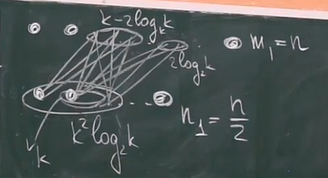
\includegraphics[width=12cm]{polina_5.PNG}
\\
\\
Пусть $m_2 = k^2log_2k, n_2 = (n - (k - 2log_2k))$
\\
Из каждой вершины верхней доли $G_{m_2, n_2}$ в нижнюю долю этого графа выходят $\geq \frac{n}{2} - (k-2log_2k)$ ребер\\
$p(G_{m_2,n_2}) \geq \frac{n/2 - k + 2log_2k}{n - k + 2log_2k} \geq \frac{n/2 - k}{n} = 1/2 - k/n = p$
\\
Снова воспользуемся леммой\\
$n_2C_{m_2/2 - m_2k/n}^{k} > (2log_2k - 1)C_{m_2}^{k} \\(1+o(1))(1+\varepsilon)log_2k2^{k+1}\frac{(k^2log_2k(1/2 - k/n))^k}{k!} > (1+o(1))(2log_2k)\frac{(k^2log_2k)^k}{k!}$
\\
\textbf{Замечание 1} Мы имели право так асимптотически оценивать $C_a^b \sim \frac{a^b}{b!}$, если $a = o(b)$. Мы прошлись по грани....
\\
\textbf{Замечание 2} $(\frac{1}{2} - \frac{k}{n})^k = (1/2)^k(1 - \frac{2k}{n}) \sim (1/2)^k$ 
\\
$(1+o(1))(1+\varepsilon) > (1+o(1))$
\\
\\
Значит, можно воспользоваться леммой, и найдется в точности подграф $K_{k,k}$
\EndProof
\newpage{}


\section{(8) Конструктивная нижняя оценка Франкла–Уилсона для $R(s, s)$. Лемма для кликового числа без доказательства.}
\section{(8) Конструктивная нижняя оценка Франкла–Уилсона для $R(s, s)$. Лемма для числа независимости без доказательства.}
$G(n, 3, 1)$ - полный граф, где вершины это тройки элементов $n$-го множества, а рёбрами соединяем две тройки, если их пересечение ровно один элемент.

$\alpha (G)$ - максимальное независимое множество графа.

$\omega (G)$ - максимальная клика графа.

$V(G)$ - количество вершин в графе.

\Statement $R(s, s) \geqslant \frac{s^3}{6} (1 + o(1))$

\Proof $\alpha (G(n, 3, 1)) \leqslant n$ (доказывалась в прошлом семестре)

$\omega (G(n, 3, 1)) = \left[ \frac{n-1}{2} \right]$

Пример клики размером $\left[ \frac{n-1}{2} \right]$:\\ 
$\{1, 2, 3\}, \{1, 4, 5\}, \{1, 6, 7\}, ...$\\
Оценка на $\omega(G(n, 3, 1))$ доказывается очень просто. Достаточно просто  рассмотреть клики устроенные по другому. 

$V(G(n, 3, 1)) = C_n^3 \thicksim \frac{n^3}{6}$ 

Получили граф на $C_n^3$, у которого $\alpha (G) < n + 1$ и $\omega (G) < n+1$

Следовательно,

$$R(n + 1, n + 1) \geqslant C_n^3$$

$$R(s, s) \geqslant \frac{s^3}{6} (1 + o(1))$$
\EndProof

\Th (Франклина, Уилсона, 1981)

$$R(s, s) > (e^{\frac{1}{4}} + o(1))^{\frac{ln^2(s)}{ln(ln(s))}}$$

\Proof

Пусть $p$ - простое число, $m = p^3,l = p^2$.

Рассмотрим граф:\\
Вершины: $V = \{\overline{x} = (x_1, ..., x_m), x_i \in \{0, 1\}, x_1 + ... + x_m = l \}\}$\\
Рёбра: $E = \{\{\overline{x}, \overline{y}\}: \overline{x} \neq \overline{y}, (\overline{x}, \overline{y}) \equiv 0 (p)\}$

Пусть $s(p) = (\sum_{k=0}^{p} C_m^k) + 1, где n = C_m^l$ ($n$ - сколько всего вершин)

\Lemma 1 (О числе независимости, б/д)
$$\alpha(G) \leqslant \sum_{k=0}^{p-1} C_m^k < s(p)$$

\Lemma 2 (О кликовом числе, б/д)
$$\omega(G) \leqslant \sum_{k=0}^{p} C_m^k < s(p)$$

Только из неравенств в леммах следует: $R(s(p), s(p)) > n$

Если мы докажем, что 
$n = n(s) = (e^{\frac{1}{4}} + o(1))^{\frac{ln^2(s)}{ln(ln(s)))}}$ ($n(s)$ - формула зависимости $n$ от $s$), тогда мы докажем теорему для всех $s = s(p)$ воспользовавшись неравенством $R(s(p), s(p)) > n$.

Если утверждение: $n(s) =  (e^{\frac{1}{4}} + o(1))^{\frac{ln^2(s)}{ln(ln(s)))}}$ для $s = s(p)$, то сможем доказать теорему для произвольного $s = s_2$: \\ 
Для этого найдём $max(p): s(p) \leqslant s_2,$ \\
тогда $R(s_2, s_2) \geqslant R(s(p), s(p)) = (e^{\frac{1}{4}} + o(1))^{\frac{ln^2(s(p))}{ln(ln(s(p))))}}$. Из этого мы хотим вывести: $R(s_2, s_2) \geqslant (e^{\frac{1}{4}} + o(1))^{\frac{ln^2(s_2)}{ln(ln(s_2)))}}$
(По словам лектора, утверждение доказывается нудно, через дважды логарифмирование выражения выше. В частности надо пользоваться тем, что простые числа плотно встречаются в натуральном ряде между $n$ и $n + o(n)$ или $n + O(n^{0.525})$ обязательно есть простое число, без этого мы не сможем доказать, что $ln(s)$ и $ln(s(p))$ ведут себя асимптотичекси одинаково).

Однако продолжим. Докажем, что $n(s) =  (e^{\frac{1}{4}} + o(1))^{\frac{ln^2(s)}{ln(ln(s)))}}$, для $s = s(p)$.

Напомню, что $s(p) = \sum_{k=0}^p C_m^k + 1, n = C_m^l$
$$n = C_{p^3}^{p^2} = \frac{p^3 (p^3 - 1) ... (p^3 - p^2 + 1)}{p^2!} = \frac{(p^{3(1+o(1))})^{p^2}}{(p^{2(1+o(1)})^{p^2}} = p^{3p^2(1 + o(1)) - 2p^2(1 + o(1))} = p^{p^2(1 + o(1))}$$ (факториал раскрыли по формуле Стирлинга) 

Поскольку $s(p) = \sum_{k=0}^p C_m^k + 1$, то

$s < (p + 1) C_m^p + 1$

$s > C_m^p + 1$

$$C_m^p = C_{p^3}^p = \frac{p^3(p^3-1)...(p^3-p+1)}{p!}= p^{3p(p+o(1))-p(1+o(1))} = p^{2p(1+o(1))}$$

$s < (p + 1) C_m^p + 1 = (p+1) p^{2p(1+o(1))} + 1 = p^{2p(1+o(1))}$

$s > C_m^p + 1 = p^{2p(1+o(1))} + 1 = p^{2p(1+o(1))}$, поэтому $s = p^{2p(1+o(1))}$

Получили $s = p^{2p(1+o(1))}, n = p^{p^2(1+o(1))} \Rightarrow$

$ln(s) = 2p(1+o(1))ln(p)$

$ln^2(s) = 4p^2 (1+o(1)))ln^2(p)$

$ln(ln(s)) = ln(2) + ln(p) + ln(1 + o(1)) + ln(ln(p)) = (1+o(1)) ln(p)$

$\frac{ln^2(s)}{ln(ln(s))} = 4p^2 ln(p)(1 + o(1))$

$ln(n) = p^2 ln(p) (1 + o(1))$

Из двух последних равенств следует: $ ln (n) \thicksim \frac{ln^2(s)}{4 ln(ln(s))} \Rightarrow n = (e + o(1))^{\frac{ln^2(s)}{4 ln(ln(s))}}$

Далее, воспользовавшись неравенством $R(s, s) > n$, получим $R(s, s) > (e + o(1))^{\frac{ln^2(s)}{4 ln(ln(s))}}$

\EndProof



\newpage{}


\section{(5) Многоцветные числа Рамсея и числа Рамсея для гиперграфов. Существование и рекуррентные верхние оценки.}
\setcounter{section}{18}

\section{Частично упорядоченные множества. Диаграмма Хассе. Изоморфизм. Описание попарно неизоморфных ч.у.м. для 3-х и 4-х элементов. Минимальные, максимальные, наибольшие и наименьшие элементы.}

Множество A с заданным на нем частичным порядком R называется \textbf{частично упорядоченным множеством (ЧУМ)} и обозначается (A; R). \textbf{Отношением (нестрогого частичного) порядка} называется любое рефлексивное, антисимметричное и транзитивное отношение. \\ \par

\textbf{Диаграммой Хассе} называется ориентированный граф без циклов, по которому отношение порядка строится так: $a \leqslant b$, если из a в b идёт ориентированный путь. Диаграмму Хассе для отношения можно получить из ориентированного графа, его изображающего, выкидыванием петель и таких рёбер между вершинами a и c, если есть вершина b, такая, что: $a < b < c$. Кроме того, вместо рисования стрелок граф располагают так, чтобы большие элементы находились выше. \par
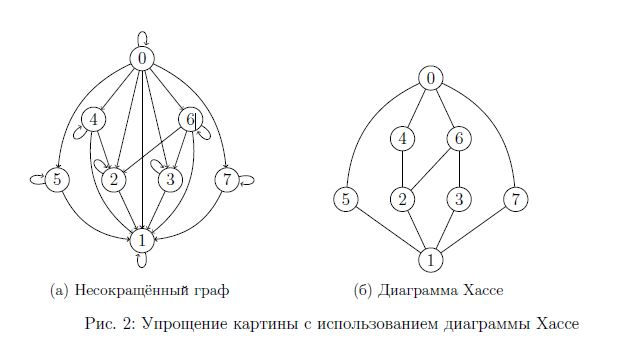
\includegraphics{images/19_hasse} \par

\textbf{Изоморфизмом} упорядоченных множеств $(A, \leqslant_A)$ и $(B, \leqslant_B)$ называется биекция $f: A \rightarrow B$, для которого выполнено свойство:  $x \leqslant_A y \Leftrightarrow f(x) \leqslant_B f(y)$. Обозначение: $A \simeq B$. \\ \par
\emph{Описание попарно неизоморфных ч.у.м. для 3-х и 4-х элементов.} Доказательство основывается на попарно неизоморфных графах без петель и кратных рёбер (для n=3 их 4, для n=4 их 11) \par
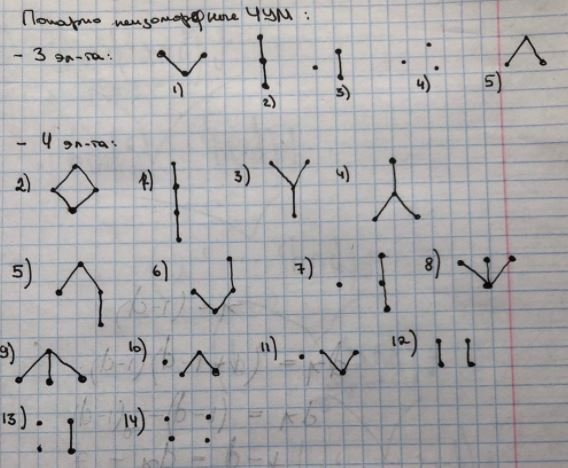
\includegraphics{images/19_pos} \\ \par

Элемент $x \in A$ \textbf{наибольший} в упорядоченном множестве $(A, \leqslant_A)$, если $\forall y \in A: y \leqslant_A x$. Элемент $x \in A$ \textbf{максимальный} в упорядоченном множестве $(A, \leqslant_A)$, если $\nexists y \in A : x <_A y$. Наименьший и минимальный элементы определяются аналогично. \\ \par

\emph{Свойства максимальных/наибольших/минимальных/наименьших элементов:} \\
1. Наибольший элемент всегда является максимальным, причём единственным; \\
2. Максимальных элементов может быть несколько; \\
3. Единственный максимальный элемент не всегда является наибольшим. \\ \par
$\blacktriangle$
1. Если x наибольший, то $x \leqslant y$ для всех $y \in A$. Поэтому $x \nless y$ для всех y. Поэтому он максимален. Любой другой элемент будет меньше наибольшего
и потому не будет максимальным. \par
2. Например, можно взять натуральные числа от 1 до 10 и отношение делимости.
Максимальными будут числа 6, 7, 8, 9, 10: на них никакое число из этого интервала
не делится. \par
3. Например, можно взять множество $\{ 3 \} \cup \{2^n | n \in \mathbb{N}\}$ с отношением делимости. 3 является единственным максимальным элементом, т.к. на любое другое делится ещё какое-то число. Но наибольшего элемента тут нет.
$\blacksquare$
\newpage{}


\section{(7) Гиперграфы. Гиперграфы $t$-пересечений. Теорема Эрдёша–Ко–Радо (о максимальном числе ребер в гиперграфе $1$-пересечений).}
\setcounter{section}{19}

\section{Диаграмма Хассе. Определение цепи и антицепи. Теорема о длине наибольшей цепи в ч.у.м. (б/д). Доказательство теоремы на примерах задач о людоедах и числах.}
\textbf{Диаграммой Хассе} называется ориентированный граф без циклов, по которому отношение порядка строится так: $a \leqslant b$, если из a в b идёт ориентированный путь. (см. билет 19) \\ \par

\textbf{Цепь упорядоченного множества $\langle M, \leqslant_M \rangle$} - упорядоченная последовательность элементов $a_1, a_2, \dots, a_n$, для которой $a_i \leqslant_M a_{i+1} $ для всех $1 \leqslant i \leqslant n-1$. \textbf{Антицепь} - набор элементов, никакие два из которых не находятся в отношении $\leqslant_M$. \\ \par
\textbf{Теорема}. Если d длина наибольшей цепи в упорядоченном множестве, то упорядоченное множество можно разбить на d антицепей. \par
\textbf{Задача 6.2 про людоедов} Некоторые людоеды хотят съесть некоторых других людоедов. Известно, что длина наибольшей
цепочки, в которой каждый людоед хочет съесть последующего, равна n (в частности, циклов нет). Докажите, что людоедов можно рассадить в n пещер, в каждой из которых никто никого не хочет съесть. Можно ли гарантированно рассадить их в меньшее число пещер? \par
$\blacktriangle$
Аналогично задаче 6.3, выбираем сначала все минимальные элементы для этого ч.у.м. Каждая следующая пещера: все людоеды, которых хотят съесть только людоеды из предыдущих пещер. Из условия, что максимальная цепь n, мы разбиваем всех великанов на n пещер, в каждой пещере антицепь. При этом гарантированно меньше пещер получить нельзя, рассмотрим пример с n великанами, где каждый великан пронумерован, и хочет съесть всех великанов с номером, большим, чем у него.
$\blacksquare$ \\ \par

\textbf{Теорема}. В упорядоченном множестве из mn + 1 элемента есть цепь длины n + 1 или антицепь из $m + 1$ элемента. \par
\textbf{Задача 6.3 про числа} (а) Докажите, что среди 36 различных натуральных чисел или найдется 6 чисел, среди которых ни одно не делится на другое, или найдется 8 чисел, которые можно выстроить в цепь, где каждое число делится на следующее. (б) Верен ли аналогичный факт для целых чисел? \par
$\blacktriangle$
(а) Пусть не найдётся ни цепь длины 8, ни антицепь длины 6. Тогда возьмём все числа, которые в данном ч.у.м. являются минимальными. Очевидно, что количество таких чисел $\leqslant 5$. Последовательно будем выбирать множества чисел, которые делятся только на числа из предыдущих множеств; получим следующую схему: \\ 
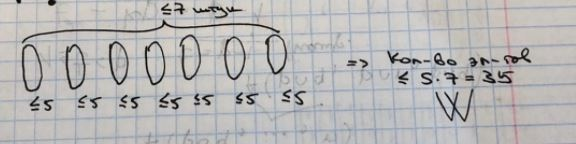
\includegraphics{images/20} \\

Нашли противоречие. Значит, начальное утверждение неверно. \\
(б) Формально, делимость среди целых чисел не является ч.у.м., т.к. нарушена антисимметричность => теорема не применима с её доказательством. Однако мы можем доопределить целые числа до ч.у.м.: будем считать, что -7 делится на 7, но не наоборот. Тогда делимость на таких целых числах будет ч.у.м. и можно применить теорему (аналогичные рассуждения из пункта а)
$\blacksquare$
\newpage{}


\section{(7) История последовательных продвижений:теорема Эрдёша–Ко–Радо (общий случай), теорема Франкла, теорема Уилсона, теорема Алсведе–Хачатряна. Все б/д, но с подробными комментариями. Нужно продемонстрировать четкое понимание, что за параметры выбираются в теореме АХ (Алсведе–Хачатрян): когда эта теорема превращается в ЭКР (Эрдеш-Ко-Радо); когда оценка становится тривиальной($C_k^n$); примеры конструкций, в которых можно явно посчитать,что оценка ЭКР не самая лучшая и АХ ее превосходит.}
1961. Теорема Эрдёш-Ко-Радо(3 математика), но сделали в 1938 году, однако не знали как применить.

$\forall r, s \exists n_0 = n_0(r, s): \forall n \geqslant n_0: f(n, r, s) = C_{r-s}^{n-s}$

1978. Теорема Франкла: Если $s \geqslant 15, r$ - любое, то $n_0(r, s) = (r-s+1)(s+1)$ (при достаточно большом $s$)

1982 Уилсон: $\forall s, r:\ n_0(r, s) = (r-s+1)(s+1)$. Для $n \geqslant n_0: f(n, k, t) = C_{n-t}^{k-t}$, а для меньших $n$: $f(n, k, t) > C_{n-t}^{k-t}$

Есть тривиальная конструкция, когда $n \leqslant 2k - s - 1$, тогда любые два подмножетсва размера $k$ пересекаются по не менее, чем $s$ элементов $\Rightarrow f(n, k, s) = C_n^k$

1996. Теорема Алсведе–Хачатряна.

Зафиксируем $r, s$. Пусть $n \geqslant 2r - s$. Выберем такое $b \in N$, что
$$(r-s+1)(2+\frac{s-1}{b+1}) \leqslant n < (r-s+1)(2+\frac{s-1}{b})$$

(При b = 0 левая часть становится как в теореме Франка-Уилсона, а правая - бесконечность. Также сводится к ЭКР)

Тогда 
$$f(n, r, s) = \left| \{F \subset \{1, ..., n\}: |F| = r \wedge |F \cap \{1, 2, ..., 2b + s\}| \geqslant b + s\} \right| = \sum_{i=b+s}^{2b+s} C_{2b+s}^i C_{n - 2b - s}^{r-i}$$ 
- Эти множества $r$ элементные и пересекаются хотя бы по $s$ элементам.

\Example $n = 8, r = 4, s = 2$. В этом случае при $b = 1$.    

$$f(8, 4, 2) = \left| \{F \subset \{1, ..., 8\}: |F| = 4, |F \cap \{1, 2, ..., 4\}| \geqslant 3\} \right| = 17$$ 

А если воспользоваться оценкой Эрдёш-Ко-Радо: $f(n, r, s) \geqslant C_{n - s}^{r - s}$

Получим $f(8, 4, 2) \geqslant C_{6}^{2} = 15 < 17$. Оценка по АХ оказалась лучше.


\newpage{}


\section{(4) Системы общих представителей (с.о.п.). «Тривиальные» нижние и верхние оценки.}
\setcounter{section}{8}
\section{Проверка правильности скобочной последовательности с несколькими типами скобок.}
\par \textbf{Определение}: \textit{Правильные скобочные последовательности с несколькими типами скобок} (рассмотрим с двумя)
\begin{enumerate}
    \item $\varepsilon$ (пустое слово) - ПСП
    \item $S$ - ПСП $\Rightarrow (S), [S]$ - ПСП
    \item $S_1, S_2$ - ПСП $\Rightarrow S_1 S_2$ - ПСП 
\end{enumerate}
\par \textbf{Задача:} Проверить, является ли последовательность из нескольких типов скобок правильной скобочной последовательностью
\par \textbf{Решение:} Храним стек незакрытых открывающих скобок
\lstinputlisting[language=C++,
emph={int,char,double,float,unsigned},
emphstyle={\color{blue}}
]{code/9_psp.cpp}
\par \textbf{Утверждение:} Данный алгоритм корректен, то есть ПСП $\Leftrightarrow$ алгоритм вывел true
\begin{itemize}
    \item[$\blacktriangle \Rightarrow$] Индукция по построению \begin{enumerate}
    \item База: $\varepsilon$ - обработается корректно
    \item $T=(u)$, $u$ - ПСП. По предположению индукции, всё $u$ удалится из стека к моменту прихода закрывающей скобки (можно считать, что стек начинается после первой скобки, она никак не влияет на применение алгоритма к $u$), а внешние скобки обработаются корректно (аналогично для других типов скобок)
    \item $T=T_1 T_2; T_1, T_2$ - ПСП. По предположению индукции, после того как считается $T_1$ стек опустошится $\Rightarrow$ после $T_2$ - тоже $\Rightarrow$ алгоритм сработает корректно $\blacksquare$
    \end{enumerate}
    \item[$\Leftarrow$] Доказываем индукцией по количеству действий, "обращая" предыдущий пункт.
    \par Рассмотрим скобочную последовательность, на которую алгоритм выдаёт true. Алгоритм сопоставил каждой открывающейся скобке одного типа закрывающуюся скобку того же типа. Причём они обязательно идут в правильном порядке. 
\parДля доказательства факта используем индукцию.
Рассмотрим пары соответсвующих скобок в порядке закрытия пары:
\begin{enumerate}
    \item База: Если между парой скобок нет других скобок, то последовательность от одной скобки до другой - правильная.
    \item Шаг: Если между парой скобок (назовём их $a$ и $b$ соответственно) есть непустая подстрока, то все скобки из подстроки уже были рассмотрены индукцией, так как открывающиеся скобки в подстроке были позже, чем $a$ добавлены в стек и по правилу стека должны были раньше из него выйти, а значит они уже были рассмотрены индукцией. Аналогично с закрывающимеся скобками из подстроки - они идут раньше, чем $b$, следовательно, по правилу стека им ставили в соответствие открывающиеся скобки, которые были добавленны позже $a$. (окрывающаяся скобка не могла быть добавленны раньше $a$, потому что $a$ перегородила бы ей выход.) По предположению индукции получаем, что подстрока состоит из одной или нескольких ПСП $\Rightarrow$ сама подстрока ПСП. $\Rightarrow$ Подпоследовательность от $a$ до $b$ - правильная. $\blacksquare$
\end{enumerate}
\end{itemize} 
\newpage{}

\section{(5) Верхняя оценка размера минимальной с.о.п. с помощью жадного алгоритма.}

\Def Пусть $S$ — полукольцо. Функция $m : S \rightarrow [0, +\infty)$ называется \textit{конечной мерой} на $S$, если выполняется свойство \textit{аддитивности}:

$\forall A, A_1, \dots , A_n \in S\ (\bigsqcup^n_{i=1} A_i = A \Rightarrow m(A) = \sum^n_{i=1} m(A_i))$

\Def $m$ называется \textit{$\sigma$-аддитивной конечной мерой} на полукольце $S$, если:
\begin{enumerate}
    \item $m$ — конечная мера на $S$
    \item $\forall A, \{A_i\}^{\infty}_{i=1} \in S\ (\bigsqcup^{\infty}_{i=1} A_i = A \Rightarrow m(A) = \sum^{\infty}_{i=1} m(A_i))$ (ряд должен сходиться)
\end{enumerate}

\Conseq (из теоремы о продолжении меры на кольцо, они будет ниже).
\begin{enumerate}
    \item Если $\bigsqcup_{i=1}^{\infty} A_i \subseteq A$, то 
$$m(A) \geq \sum^{\infty}_{i=1} m(A_i)$$
    \item Если $A \subseteq
\bigcup_{i=1}^n A_i$, то 
$$m(A) \leq \sum^n_{i=1} m(A_i)$$
    \item $m$ - $\sigma$-аддитивна, если $A \subseteq \bigcup^{\infty}_{i=1} A_i$, то $$m(A) \leq \sum^{\infty}_{i=1} m(A_i)$$
\end{enumerate}
\Proof
Пусть $\nu$ - продолжение меры $m$ на $R(S)$.
\begin{enumerate}
    \item $m(A) = \nu(A) = \nu((\bigsqcup^n_{i=1} A_i) \sqcup (A \backslash (\bigsqcup^n_{i=1} A_i))) = \sum^n_{i = 1} \nu(A_i) + \nu(A \backslash (\bigsqcup^n_{i=1} A_i)) \geq \sum^n_{i = 1} \nu(A_i) = \sum^n_{i = 1} m(A_i)$. Следовательно, по теореме о предельном переходе:
    $$m(A) \geq \sum^{\infty}_{i=1} m(A_i)$$
    
    \item $B_1 = A_1 \cap A$.
    $B_i = (A_i / \bigcup_{j = 1}^{i-1} A_j) \cap A$
    Тогда $A = \bigsqcup_{i=1}^n B_i$
    
    $$\nu(A) = \sum^{n}_{i = 1}\nu(B_i) \leq \sum^{n}_{i = 1}\nu(A_i)$$
    
    \item Абослютно такое же. Но будет бесконесчно много $B_i$, а вместо $n$ должно быть $\infty$. 
    
\end{enumerate}

\leftbar

\LemmaN{1} Если $m$— мера на полукольце $S$, и множества $A, A_1, \dots , A_n \in S$ таковы, что $A \subset
\bigcup_{i=1}^n A_i$, то 
$$m(A) \leq \sum^n_{i=1} m(A_i)$$

\Proof По ранее доказанной лемме существует такой набор попарно непересекающихся множеств $B_1, \dots, B_q$, что любое множество из $\{A, A_1, \dots , A_n\}$ представимо как объединение некоторых элементов набора (можно считать, что $\forall B_i\ \exists A_j\ (B_i \subseteq A_j ))$. Далее,

$$\bigcup^n_{i=1} A_i = \bigsqcup_{i=1}^q B_i \supset A$$

$$\sum^n_{i=1} m(A_i) = \sum^n_{i=1} \sum_{j:B_j \subseteq A-i} m(B_j) \geq \sum^q_{k=1} m(B_k) \geq m(A)$$ \EndProof

\LemmaN{2} Если $m$ — мера на полукольце $S$, и множества $A, A_1, \dots , A_n \in S$ таковы, что $A_i$ попарно не пересекаются, и $A_i \subset A$, то 
$$m(A) \geq \sum^n_{i=1} m(A_i)$$

\Proof По определению полукольца набор $\{A_i\}$ можно “дополнить до $A$”, а дальше всё очевидно. \EndProof

\Conseq С помощью предельного перехода данную лемму можно обобщить на бесконечный набор $\{A_i\}$.
\endleftbar

\Example 

(Классическая мера Лебега на полукольце промежутков и ее сигмааддитивность) Промежутки в $\mathbb{R}$ образуют полукольцо, на котором длина промежутка является мерой.

\Th Длина промежутка — $\sigma$-аддитивная мера.

%\begin{enumerate}
\Proof 

1) Пусть $\lfloor a, b \rceil = \bigsqcup^{n}_{i=1} \lfloor a_i, b_i \rceil$ — некоторый промежуток. ($a = a_1, b_1 = a_2, b_2 = a_3, \dots, b_n = b$)

Тогда $m(\lfloor a, b \rceil) = b - a = \sum^n_{i=1}(b_i - a_i) = \sum^n_{i=1} m(\lfloor a_i, b_i \rceil)$

2) Пусть $\lfloor a, b\rceil = \bigsqcup^{\infty}_{i=1} \lfloor a_i, b_i \rceil$ — некоторый промежуток.

Формулировка леммы о конечном покрытии (принцип Гейне-Бореля): 

$I$ - отрезок, $\{U_{\alpha}\}$ - семейство интервалов. $I \in \bigcup U_{\alpha} \rightarrow \exists U_1, \dots, U_n$, т.ч. $I \subset \bigcup_{i=0}^n U_i$

Продолжим,

\begin{enumerate}

\item Возьмём такой отрезок $[\alpha, \beta] \subseteq \lfloor a, b \rceil$, что $m[\alpha, \beta] > m \lfloor a, b\rceil - \frac{\epsilon}{2}$.

\item Определим такие интервалы $(\alpha_i, \beta_i) \supseteq \lfloor a_i, b_i\rceil,$ что $m(\alpha_i, \beta_i) < m\lfloor a_i, b_i\rceil + \frac{\epsilon}{2^{i+1}}.$

\item Так как $[\alpha, \beta] \subseteq \cup^{\infty}_{i=1} (\alpha_i, \beta_i)$, то по лемме Гейне-Бореля существует конечное подпокрытие (пусть это будут интервалы $\{(\alpha_i, \beta_i)\}^k_{i=1})$
\end{enumerate}

Далее,
$$m\lfloor a, b\rceil < m[\alpha, \beta] + \frac{\epsilon}{2} \leq \sum^k_{j=1} m(\alpha_j, \beta_j) + \frac{\epsilon}{2}$$ 
$$\leq
\sum^{\infty}_{j=1} m(\alpha_j, \beta_j) + \frac{\epsilon}{2} \leq \sum^{\infty}_{j=1} m \lfloor a_i, b_i\rceil + \epsilon$$

Устремляя $\epsilon$ к нулю, получаем $m\lfloor a, b\rceil \leq \sum^{\infty}_{j=1} m\lfloor a_i, b_i\rceil$. Равенство $m\lfloor a, b\rceil = \sum^{\infty}_{j=1} m\lfloor a_i, b_i\rceil$ получается по следствию 1 в начале билета (или по следствию из леммы 2). \EndProof
%\end{enumerate}

\leftbar
\Example Полукольцо полуинтервалов $(a, b]$, мерой на котором является $m(a, b] = \phi(b) - \phi(a)$, где $\phi$ — ограниченная неубывающая непрерывная справа функция.

\Th Указанная мера является $\sigma$-аддитивной.

Доказательство для ограниченных полуинтервалов. \Proof Каждый полуинтервал
$(A_i, B_i]$ из разбиения можно покрыть интервалом $(\alpha_i, \beta_i)$, где $\alpha_i = A_i и \beta_i-B_i < \frac{\epsilon}{2} i;$ эти интервалы покрывают произвольный подотрезок. Дальнейшее доказательство аналогично предыдущему. \EndProof
\endleftbar

\newpage{}


\section{(8) Конструктивная нижняя оценка размера минимальной с.о.п.}
\Th $\forall n \geqslant 4 \forall k \leqslant \frac{n}{4} \forall s : 2 \leqslant ln \frac{sk}{n} \leqslant k$: $\exists M: \tau (M) \geqslant \frac{1}{32} \cdot  \frac{n}{k} ln \frac{sk}{n}$

Будем пользоваться неравенством $[x] \geqslant \frac{x}{2}$.

\Proof Пусть $m = [\frac{1}{2} ln \frac{sk}{n}] \geqslant 1$. Рассмотрим $N_1, \dots, N_{C_{2m}^m} \subset \{ 1, 2, \dots, 2m\} \subset \{1, 2, \dots, n\} = R_n$, где $N_i$ - все возможные m-элементные подмножества, $|N_i| = m$. 

$\tau (\{N_1, \dots, N_{C_{2m}^m}\}) = m + 1$, потому что если взять любое m-эл. мн-во найдётся обратное к нему. 

$q = [\frac{2k}{m}]; \frac{k}{m} \geqslant \frac{2k}{ln \frac{sk}{n}} \geqslant 2 \Rightarrow q \geqslant 4$

Разобьем на такие множества размера $2m$.
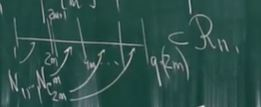
\includegraphics[]{images/est2.JPG}

В каждое разбиение размера $2m$ запихиваем совокупность выше ($N_1, \dots, N_{C_{2m}^{m}}$).

Рассмотрим множества $L_1 = N_1^1 \cup N_1^2 \cup \dots N_1^q$; $\dots$ $L_{C_{2m}^{m}} = N_{C_{2m}^{m}}^1 \cup N_{C_{2m}^{m}}^2 \cup \dots N_{C_{2m}^{m}}^q$; $ \forall i |L_i| = q\cdot m = [\frac{2k}{m}] \cdot m \geqslant \frac{k}{m} \cdot m = k$

$\tau (\{L_1, \dots, L_{C_{2m}^{m}}) = m + 1$ (очевидно, т.к. объединения одинаковые, сохраняется предыдущий результат для $\tau$).

$C_{2m}^m < 2^{2m} \leqslant 2^{ln \frac{sk}{n}} < e^{ln \frac{sk}{n}} = \frac{sk}{n}$

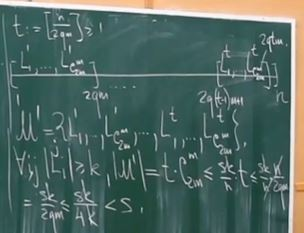
\includegraphics[]{images/est3.JPG}

$\tau(M') = t(m+1) > tm \geqslant \frac{n}{4qm} m \geqslant \frac{nm}{8k} \geqslant \frac{1}{32} \frac{n}{k} ln \frac{sk}{n}$. Но если какое-то из множеств мощности больше, чем k, то просто удалим из него любые элементы (соп от этого не уменьшится). $\tau(M'') \geqslant \tau(M')$
\EndProof
\newpage{}

\section{(10) Вероятностная нижняя оценка размера минимальной с.о.п. Следствие из неё.}
\Th Пусть для данных $n, k, s$ l: 
\[ C_n^l \cdot \frac{C_{C_n^k - C_{n-l}^k}^s}{C_{C_n^k}^{s}} < 1\]
Тогда $\exists M: \tau(M) > l$

\Proof
Рассмотрим случайное $M = \{M_1, \dots, M_s \}$; количество таких совокупностей - ${C_{C_n^k}^{s}}$. Фиксируем $L \subset R_n, |L| = l$. 

$P(L$ является с.о.п. для $M) = \frac{C_{C_n^k - C_{n-l}^k}^s}{C_{C_n^k}^{s}}$

$P(\exists L, |L| = l: L $ явл. с.о.п. для $M) \leqslant C_n^l \cdot \frac{C_{C_n^k - C_{n-l}^k}^s}{C_{C_n^k}^{s}} < 1$ (по усл. теоремы), значит $\exists M:$ у $M$ нет $l$ - элементных с.о.п.
\EndProof

\Cor \Th Пусть $n \to \infty$, $s=s(n), k=k(n) \to \infty, \frac{sk}{n} \to \infty$

Пусть $ln ln (k) = o(ln \frac{sk}{n}), ln^2 \frac{sk}{n} = o(k), k^2 = o(n)$. 

Тогда $\exists n_0 \forall n > n_0 \exists M: \tau(M) \geqslant \frac{n}{k} ln \frac{sk}{n} - \frac{n}{k} ln ln \frac{sk}{n} - \frac{n}{k} ln ln (k) - \frac{3n}{k} \sim \frac{n}{k} ln \frac{sk}{n}$

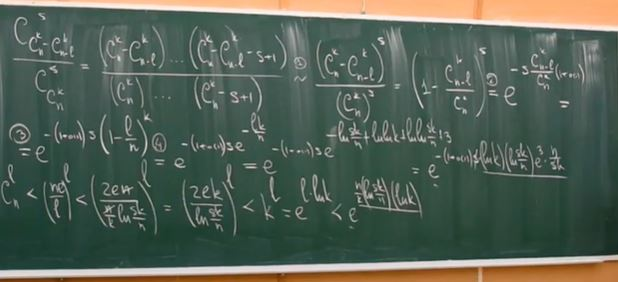
\includegraphics[width=9cm]{images/est4.JPG}

Осталось перемножить е в степенях и понять, что это стремится к нулю, значит, начиная с какого-то $n_0$ оно будет меньше 1.

Проверим переходы:

1) - тут на самом деле верхняя оценка и её достаточно. Ура.

2) - 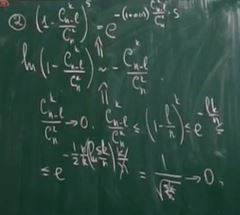
\includegraphics[width=5cm]{images/est6.JPG}

3) - тут надо в ориниальном переходе в правой части поставить $\leqslant$ и вместо $(1 - \frac{l}{n})^k$ написать $(1 - \frac{l}{n-k})^k$.

4) - 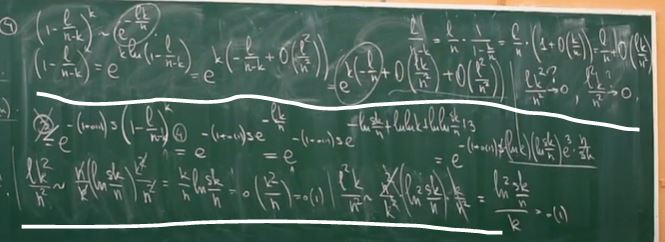
\includegraphics[width=9cm]{images/est7.JPG}
\newpage{}

\section{(7) Нижняя оценка размера минимальной с.о.п. с помощью обобщенных с.о.п. Не требуется проверять, то что определенное значение $\ell$ подходит под условие теоремы.}

\Th Пусть даны $n, k, s$. Рассмотрим произвольное $\ell$, обозначим $n' = C_n^k, s' = C_n^{\ell}, k' = C_{n - \ell}^k$. Предположим, что для $\ell$ выполнено неравество:

$$
max\{ \frac{n'}{k'}, \frac{n'}{k'} ln\bigg(\frac{s' k'}{n'}\bigg)\} + \frac{n'}{k'} + 1 \leq s
$$

Тогда $\exists \mathcal{M} = \mathcal{M}(n, k, s): \ \tau(\mathcal{M}) > \ell$.

\Proof Зафиксируем $n, s, k$. Мы хотим построить $\mathcal{M} = \{M_1, M_2, \ldots, M_s\}$ такие, что $\forall i \in \{1, \dots, s\}: \ |M_i| = k, M_i \subseteq \{1, 2, \ldots, n\}: \ \tau(M) > \ell$, то есть нужно, чтобы было верно следующее: 

$$
\forall L \subset \{1, 2, \ldots, n\}: \ |L| = \ell \ \exists M_i \in \mathcal{M}: \ M_i \cap L = \varnothing \Longleftrightarrow M_i \subset \{1, 2, \ldots, n\} \setminus L
$$

То есть нам надо выбрать с.о.п. для каждого $n - \ell$ элементного множества, при этом их должно оказаться не больше $s$. 

Далее для всех $(n-\ell)$-элементных подмножеств $\{1, \ldots, n\}$ мы хотим рассматривать все $k$-элементные множества, которые лежат в них целиком.

Давайте рассмотрим все $k$-элементные подмножества, обозначим их за $K_1, \ldots, K_{C_n^k}$. Перейдем от $K_i$ к их номерам, то есть далее каждому множеству будет сопоставляться число. Рассмотрим каждое $(n - \ell)$ элементное подмножество $L_j : j \in \{1, \ldots, C_n^{\ell}\}$. Их всего $C_n^{n - \ell} = C_n^{\ell}$. Теперь рассмотрим все такие $i$, что $K_i \subset L_j$, то есть множество представителей $L_j$. Таких $i$ будет $C_{n-\ell}^k$, они образуют подмножество в множестве $\{1, 2, \ldots, C_n^k\}$, множество из таких $K_i$ обозначим за $\Lambda_i$.

Теперь заметим, что у нас есть множество $\{1, 2, \ldots, C_n^k\}$ и есть $C_n^{\ell}$ модмножеств из $C_{n - \ell}^k$ элементов, при этом для нее нам надо построить с.о.п. Переобозначим $n' = C_n^k, s' = C_n^{\ell}, k' = C_{n - \ell}^k$. Теперь возьмем любую минимальную с.о.п. для совокупности $\Lambda_1, \ldots, \Lambda_{s'}$. Обозначим ее за $\sigma_1, \ldots, \sigma_{\tau}$. 

По определению с.о.п. 

$$\forall j \in \{1, \ldots, s'\} \ \exists i: \ \sigma_i \in \Lambda_j \Longleftrightarrow \forall j \in \{1, \ldots, s'\} \ \exists i: \ K_{\sigma_i} \subset L_j$$

Рассмотрим $\mathcal{M} = \{K_{\sigma_1}, \ldots, K_{\sigma_{\tau}}\}, \ \tau(\mathcal{M}) > \ell$. Тогда это искомая с.о.п., чей размер оценивается жадным алгоритмом:

$$
\tau(\mathcal{M}) \leq max\{ \frac{n'}{k'}, \frac{n'}{k'} ln\bigg(\frac{s'k'}{n'}\bigg)\} + \frac{n'}{k'} + 1 = max\{ \frac{C_n^k}{C_{n - \ell}^k}, \frac{C_n^k}{C_{n - \ell}^k} ln\bigg(\frac{C_n^{\ell} C_{n - \ell}^k}{C_n^k}\bigg)\} + \frac{C_n^k}{C_{n - \ell}^k} + 1
$$

Что, очевидно, не больше, чем $s$, так как $\tau(\mathcal{M}) \leq |\mathcal{M}| = s$. Теорема доказана.

\EndProof
\newpage

\section{(7) С.о.п. в геометрии (теорема о треугольниках на плоскости, б/д). Размерность Вапника–Червоненкиса. Теорема Радона (б/д). Подсчет размерности семейства полупространств. Лемма о числе областей в пространстве заданной мощности и размерности. Лемма о размерности измельчения (достаточно доказать существование верхней оценки, не обязательно такой, как на лекции)}

\textbf{С.о.п. в геометрии}

Рассмотрим множество точек $S \subset \mathbb{R}^2$ конечной мощности. Начнем пересекать его cо всевозможными треугольниками в этой плоскости и пусть $\mathcal{M}$ это система всех подмножеств $S$, которые можно получить, пересекая $S$ с треугольниками. 

Зафиксируем теперь $\varepsilon \in (0, 1)$ и пусть $\mathcal{M}_\varepsilon \subseteq \mathcal{M} = \{ M \in \mathcal{M} \mid |M| \geqslant \varepsilon|S| \}$

\Th (Вапника-Червоненкиса, частный случай) $\forall \varepsilon\:\: \exists \text{с.о.п.} N $ для совокупности $\mathcal{M}_\varepsilon$, такая что $$ |N| \leqslant \frac{500}{\varepsilon} \log_2 \frac{500}{\varepsilon}$$

\Note Мощность $N$ не зависит от $S$ и $n$.\\

\textbf{Размерность Вапника-Червоненкиса. Теорема Радона (б/д).}\\

\Def Пара $(\mathcal{X},\: R)$, где $\mathcal{X}$ -- произвольное множество, а $R \subseteq 2^{\mathcal{X}}$,  называется {\it ранжированным пространством}. \\ 

\Def Подмножество $A \subseteq \mathcal{X}$ {\it дробится} системой $R$, если $$\forall B \subseteq A\:\: \exists r \in R:\:\: A\cap r = B,$$
причем \textit{проекцией} системы $R$ на $A$ назовем множество $Pr_A R = \{ r \cap A \mid r \in R\}$ всевозможных пересечений $r\in R$ с $A$. Очевидно, что $A$ дробится тогда и только тогда, когда $Pr_A R = 2^A$.

\Def \textit{Размерность Вапника-Червоненкиса} $VC(\mathcal{X}, R)$ ранжированного пространства $(\mathcal{X}, R)$ по определению равна$$ VC(\mathcal{X}, R) := \max \{m \in \mathbb{N}\: \mid\: \exists A \subseteq \mathcal{X},\: |A| = m:\:\: Pr_A R = 2^A \}$$
    (если такого $m$ не существует, то $VC(\mathcal{X}, R) = +\infty$).

\Example $VC(\mathbb{N}, 2^{\mathbb{N}}) = +\infty$.

\Example $VC(\mathbb{R}, \mathcal{H}) = 2$, где $\mathcal{H}$ --- семейство всех лучей

\Th (Радон, б/д)\\
Любое множество из $n+2$ точек $S \subset \mathbb{R}^n$ можно представить как $S = A_1 \sqcup A_2$, причем выпуклые оболочки $A_1$ и $A_2$ пересекаются, т.е. $$ conv(A_1) \cap conv(A_2) \neq \varnothing.$$ 

\textbf{Подсчет размерности семейства полупространств.}\\

\Statement $VC(\mathbb{R}^n, \mathcal{H}) = n + 1$, где $\mathcal{H}$ --- семейство всех открытых полупространств (например для $n=2$ это полупоскости).

\Proof Поскольку $n+1$ вершина симплекса в $\mathbb{R}^n$ дробится, то верно неравенство $VC(\mathbb{R}^n, \mathcal{H}) \ge n+1$. \\ Для множества $S,\: |S| \ge n+2$ найдем предстваление $A_1 \sqcup A_2$ из теоремы Радона. Тогда очевидно, что отдробить $A_1$ не получится.

\EndProof

\textbf{Лемма о числе областей в пространстве заданной мощности и размерности.}

\Lemma \textbf{(1)} Пусть $(\mathcal{X},\: R)$ --- ранжированное пространство, такое что $VC(\mathcal{X}, R) = d,\:\: |\mathcal{X}| = n$. Тогда верно неравенство $$ |R| \le g(n, d) = \sum\limits_{i=0}^{d} C_n^i.$$

\Proof Заметим сначала, что $g(n, d) = g(n-1, d) + g(n-1, d-1)$ --- следствие из треугольника Паскаля.\\
Воспользуемся индукцией по $n$ и $d$. \\

\textit{База:} 

Пусть $n=0$ и $d$ произвольное. Тогда $R$ равно либо $\{ \varnothing\}$, либо $\varnothing$. В любом случае, $|R| \le 1$. В то же время, очевидно, что $VC(\mathcal{X}, R) \le n = 0$. Но тогда $|R| \le 1 = g(0, 0)$. 

Пусть, наоборот, $d=0$ и $n \ge 1$ --- произвольное. Предположим, что $|R| \ge 2$. Тогда $\exists \: R_1 \neq R_2 \in R$, причем либо в $R_1 \setminus R_2$, либо в $R_2 \setminus R_1$ содержится элемент $x \in \mathcal{X}$. Тогда множество $A = \{ x\}$ дробится $R_1$ и $R_2$, что противоречит $d=0$. Получаем $|R| \le 1 = g(n, 0)$, и база доказана. \\

\textit{Переход:} зафиксируем $(\mathcal{X}, R)$ с $VC(\mathcal{X},R) = d \ge 1$ и $|\mathcal{X}| = n \ge 1$. Рассмотрим произвольный $x \in \mathcal{X}$ и определим пространства $(\mathcal{X}_1,\: R_1),\: (\mathcal{X}_2,\: R_2)$ следующим образом:
\begin{align*}
    & \mathcal{X}_1 = \mathcal{X}_2 = \mathcal{X} \setminus \{ x\}\\
    & R_1 = \{r \setminus \{ x\}\: \mid\: r \in R\},\: R_2 = \{r \in R\: \mid\: x\not\in r\text{, но } r\cup\{x\} \in R\}
\end{align*}

Тогда имеем $|R| = |R_1| + |R_2|$. Докажем два неравенства:
\begin{enumerate}
    \item $VC(\mathcal{X}_1, R_1) \le d$ --- очевидно. Тогда по предположению индукции $|R_1| \le g(n-1, d)$.
    \item $VC(\mathcal{X}_2, R_2) \le d-1$.
    \Proof
    Предположим $VC(\mathcal{X}_2, R_2) \ge d$ и рассмотрим $A \subseteq \mathcal{X}_2,\: |A| = d,\: Pr_{R_2} A = 2^A$. По определению $R_2$, множество $A \cup \{x\}$ дробится системой $R$, но $|A \cup \{ x \}| \ge d+1$, что противоречит $VC(\mathcal{X}, R) = d$.
    \EndProof
    
    Тогда по предположению индукции $|R_2| \le g(n-1, d-1)$
\end{enumerate}

Отсюда следует, что $$|R| = |R_1| + |R_2| \le g(n-1, d) +  g(n-1, d-1) = g(n, d).$$

\EndProof

\textbf{Лемма о размерности измельчения}


\Def $h \in \mathbb{N}$. Тогда $h-$\textit{измельчение} $R$ это множество $$R_h := \{r_1 \cap \ldots \cap r_h:\: r_i \in R\}$$ 

(множества в пересечении не обязательно различные)

\Example Для $(\mathbb{R}^n, \mathcal{H})$ измельчение $R_h$ целиком содержит в себе совокупность всех выпуклых многогранников в $\mathbb{R}^n$, имеющих $h$ граней. Для $h = 3, n = 2$ это все треугольники на плоскости.

\Lemma \textbf{(2)} Пусть $d \ge 2,\: h \ge 2$ (эти ограничения наложим для удобства доказательства, остальные случаи очевидны) и $VC(\mathcal{X}, R) \le d$. Тогда $$ \exists N: VC(\mathcal{X}, R_h) \le N $$ (на лекции $N =  2dh \log_2 dh$) 

\Proof Зафиксируем любое $S \subseteq \mathcal{X}$, имеющее $|S| = n$ (на лекции было $n > 2dh \log_2 dh$) и дробящееся $R_h$ (если такое существует). По лемме (1) имеем $|Pr_R S| \le g(n, d)$. Тогда $$\left| Pr_S R_h\right| \le | Pr_S R|^h \le n^{dh}.$$
Поскольку $n \ge 2d$, то в сумме $g(n, d)$ максимально последнее слагаемое и $g(n, d) \le n^d$ ({\it б/д, по индукции}).
Поскольку  $|Pr_S R_h | = 2^n$, то должно быть выполнено неравенство $$2^n = | Pr_S R_h| \le | Pr_S R|^h \le n^{dh},$$
что неверно при достаточно больших $n$ (на лекции -- для $n > 2dh \log_2 dh$), и множества $S$ с $|S| = n$, дробящегося $R_h$, не существует.

\EndProof

\newpage{}

\section{(10) Эпсилон-сети. Теорема Вапника–Червоненкиса об эпсилон-сетях (первая лемма – только формулировка, вторая лемма с доказательством, завершение доказательства) и теорема о треугольниках как частный случай.}
\subsection{28. Алгоритм разбора по LR-таблице. Структура стека. Корректность и полнота разбора (на отл).}
\par Пусть у нас есть готовая LR-таблица table и дано слово $w=w_1 \ldots w_n\$$. Создаем стек: изначально записываем в него 0 - номер правила $S' \rightarrow S$, так как оно всегда первое в нашем выводе. Дальше запускаем цикл \begin{enumerate}
    \item Если последний символ на стеке - это номер правила ($i$), то пытаемся дописать на стек следующую букву слова $w_j$: проверяем, если в ячейке $[i, w_j]$ стоит пометка $shift$ (то есть из текущего состояния есть переход по этой букве), то дописываем эту букву на стек, иначе говорим, что слово не лежит в языке.
    \item Берем последние 2 символа со стека: среди них гарантированно одна буква ($c$) и одно число ($k$). Смотрим в ячейку $[k, c]$ \begin{enumerate}
        \item Если там стоит $(shift, to)$, то дописываем на стек $to$ - номер состояния в который надо перейти
        \item Если там стоит $(reduce, rule)$, то находим правило под номером $rule$, удаляем со стека $2 \cdot |rule.right|$ символов (нужно удалить все буквы из этого правила, но на стеке они чередуются с цифрами, поэтому умножаем длину на 2)  и дописать $rule.left$. Если делаем свертку по 0 правилу $S' \rightarrow S$, то есть в этой ячейке стоит Accept, то говорим, что слово лежит в языке.
        \item Если там стоит Error, то слово не лежит в языке
    \end{enumerate}
\end{enumerate}
\par Из алгоритма видно, что на стеке чередуются буквы и числа (в самом начале число)
\newpage{}

\section{Тема 29}
Оставлена читателям как простое упражнение.
\newpage{}

\section{(4) Размерность Вапника–Червоненкиса. Теорема Вапника–Червоненкиса (б/д). Приложения в статистике: равномерная сходимость в ЗБЧ (УЗБЧ) (б/д).}

\Def Пара $(\mathcal{X},\: R)$, где $\mathcal{X}$ -- произвольное множество, а $R \subseteq 2^{\mathcal{X}}$,  называется {\it ранжированным пространством}. \\ 

\Def Подмножество $A \subseteq \mathcal{X}$ {\it дробится} системой $R$, если $$\forall B \subseteq A\:\: \exists r \in R:\:\: A\cap r = B,$$
причем \textit{проекцией} системы $R$ на $A$ назовем множество $Pr_A R = \{ r \cap A \mid r \in R\}$ всевозможных пересечений $r\in R$ с $A$. Очевидно, что $A$ дробится тогда и только тогда, когда $Pr_A R = 2^A$.

\Def \textit{Размерность Вапника-Червоненкиса} $VC(\mathcal{X}, R)$ ранжированного пространства $(\mathcal{X}, R)$ по определению равна$$ VC(\mathcal{X}, R) := \max \{m \in \mathbb{N}\: \mid\: \exists A \subseteq \mathcal{X},\: |A| = m:\:\: Pr_A R = 2^A \}$$
    (если такого $m$ не существует, то $VC(\mathcal{X}, R) = +\infty$).
    
\Th (Вапника-Червоненкиса)
$VC(X, R) \le d \Rightarrow \forall \varepsilon \in (0, 1) \ \exists \varepsilon-\text{сеть размера} \le \lceil\frac{8d}{e}log_2{\frac{8d}{e}}\rceil$

\textbf{Напоминание ЗБЧ и УЗБЧ для испытаний Бернулли:}
$A_1, \ldots, A_n, \ldots$ -- независимые в совокупности события

$\forall i: P(A_i) = p:$

$\frac{I_{A_1} + \ldots + I_{A_n}}{n} \stackrel{p}{\longrightarrow} p$ (ЗБЧ)

$\frac{I_{A_1} + \ldots + I_{A_n}}{n} \stackrel{\text{п.н.}}{\longrightarrow} p$ (УЗБЧ)

\textbf{Про мат. статистику}

У нас есть выборка -- набор чисел $x_1, \ldots, x_n$, которые мы пронаблюдали. Мы считаем, что за этими числами стоят какие-то случайные величины $\xi_1, \ldots, \xi_n$, и эти числа служат просто их реализацией.

Эти случайные величины $\xi_1, \ldots, \xi_n$ независимы и одинаково распределены.

$F_{\xi_i}(x)$ -- функция распределения для $i$ случайной величины. Поскольку они все одинаковы, то и функция для них одна и та же. Но мы ее не знаем и хотим аппроксимировать. И вот об этом теорема Гливенко-Кантелли. В ней мы простейшим образом пытаемся приблизить функцию распределения (ступенечками).

Определим $\hat{F}_n(x_1, \ldots, x_n; x) = \frac{1}{n} \sum\limits_{i=1}^{n}I_{\{x_i \le x\}}$ ($A_j := \{x_j \le x\}$). 

УЗБЧ гласит, что $\hat{F}_n(x_1, \ldots, x_n; x) \stackrel{\text{п.н.}}{\longrightarrow} P(\xi_i \le x) = F_{\xi_i}(x)$

\Th (Гливенко-Кантелли)

$$P(sup_{\{x \in \mathbb{R}\}} \mid \hat{F}_n(x_1, \ldots, x_n; x) - F_{\xi_1}(x)\mid \xrightarrow[{n\rightarrow \infty}]{} 0) = 1$$

Переформулируем в терминах индикаторов:

$$A_1^x, \ldots, A_n^x : A_i^x = \{\xi_i \le x\}, x \in \mathbb{R}$$

$\forall x : A_i^x$ взаимно нез. и $\forall i : P(A_i^x) = p^x$

\Th (Вапника-Червоненкиса, применительно к вероятности, мб не нужна, но я оставлю)

Пусть $x \in \mathcal{X}$. Рассмотрим последовательность событий $A_1^x, \ldots, A_n^x, \ldots$ на некотором вероятностном пространстве, для которой $\forall x : A_i^x$ независимы в совокупности и $\forall x \forall n \ P(A_n^x) = p^x$.

Тогда $\frac{1}{n} \sum\limits_{i=1}^{n} I\{A_i^x\}$ сходится по $x$ равномерно к $p^x$ 

(а именно, $P(sup_{x \in \mathcal{X}} \mid \frac{1}{n} \sum\limits_{i=1}^{n} I\{A_i^x\} - p^x \mid \rightarrow 0) = 1$) тогда и только тогда, когда
$$VC(\mathcal{X};\{A_1^x, \ldots, A_n^x, \ldots \}) < + \infty$$.

\newpage{}

\section{(5) Системы различных представителей. Теорема Холла.}

\textbf{Системы различных представителей}

\Def Пусть дан набор $\mathcal{M}$ множеств. В каждом из множеств выбрали по элементу. Если все элементы различны, то такой набор назовем \textit{системой различных представителей (сокращенно с.р.п.)}. \par
Или, формально, \textit{системой различных представителей для набора $\mathcal{M}$ множеств} называется упорядоченный набор различных элементов $x(S) \in S, S \in \mathcal{M}$, т. е., такое инъективное отображение $x : \mathcal{M} \rightarrow \bigcup\limits_{S \in \mathcal{M}}S$, что $x(S) \in S$ для любого $S \in \mathcal{M}$.\\

\Th \textit{(Холла)} Пусть $S_1, \ldots, S_m$~--- конечные множества. В каждом из них можно выбрать по элементу $x_i \in S_i$ так, чтобы все $x_i$ были различны, тогда и только тогда, когда для каждого $k \in \{1, \ldots, m\}$ объединение любых $k$ из этих множеств состоит из не менее $k$ элементов.

\begin{itemize}
    \item[$\Rightarrow$] Допустим нашлись такие различные элементы $x_1, \ldots, x_m$. Тогда рассмотрим $k$-элементное подмножество $\{i_1, \ldots, i_k\} \subset \{1, \ldots, m\}$. Тогда в множестве $A = \bigcup\limits_{n = 1}^k S_{i_n}$ будут обязательно лежать элементы $x_{i_1}, \ldots, x_{i_k}$. Так как они различны, то мощность множества $A$ хотя бы $k$.
    \item[$\Leftarrow$] Индукция по $m$. База очевидна. Предположим, что для всех систем с меньшим количеством элементов утверждение верно. Пусть найдётся такое множество $I \subsetneq \{1, \dots, m\}$, что $|\bigcup\limits_{i \in I} S_i| = |I|$. Применим предположение индукции для $S_I := \{S_i | i \in I\}$. Далее, пересечения множеств из $S_{\{1, \ldots, m\} \setminus I}$ со множеством $(\bigcup\limits_{i = 1}^m S_i) \setminus (\bigcup\limits_{i \in I} S_i)$ <<непокрытых>> элементов образуют систему, для которой выполнено условие леммы Холла. Значит, можно применить предположение индукции.

    Если же такого множества $I$ не найдётся, возьмём произвольный элемент $x$ произвольного множества $S_k$. Дополнения оставшихся множеств до этого элемента образуют систему, для которой выполнено условие леммы Холла. Значит, можно применить предположение индукции.
\end{itemize}
\newpage{}

\section{(4) Перманент. Формула разложения по строке. Связь с количеством систем различных представителей.}

\Def \textit{Перманент} квадратной матрицы $A = (a_{ij})$ размера $n \times n$ определяется формулой:
$$Per(A) := \sum \limits_{\sigma \in S_n}\prod \limits_{i=1}^n a_{i,\sigma(i)},$$
где $S_n$ есть множество всех перестановок $n-$элементного множества.

Формула перманента матрицы отличается от определителя матрицы отсутствием умножения на знак перестановки.

\Def \textit{Подматрицей} данной матрицы называется матрица, полученная из данной вычеркиванием некоторого количества строк и столбцов. Перманент прямоугольной матрицы $A^{m \times n}$ определяется как сумма перманентов всех квадратных подматриц максимального размера. Или, формулой, при $m < n$:
$$Per(A) := \sum \limits_{\sigma}\prod \limits_{i=1}^m a_{i,\sigma(i)},$$
где сумма берется по всем $m-$элементным размещениям чисел от 1 до $n$. При $m > n$ положим $Per(A) = Per(A^T)$

\Th \textit{(Формула разложения по строке)} Если $m \leq n$, то для любого $i \in \{1, \ldots, m\}$
$$Per(A) = \sum \limits_{j=1}^n a_{ij}Per(A_{ij}),$$
где $A_{ij}$~--- матрица, получаемая из исходной вычеркиванием $i-$ой строки и $j-$ого столбца.

Доказательство очевидно -- просто перегруппировать слагаемые в сумме.\\

\textbf{Связь с количеством систем различных представителей}\\

\Def Пусть дан набор $\mathcal M$ множеств. В каждом из множеств выбрали по элементу. Если все элементы различны, то такой набор назовем \textit{системой различных представителей (сокращенно с.р.п.)}.

Или, формально, \textit{системой различных представителей для набора $\mathcal{M}$ множеств} называется упорядоченный набор различных элементов $x(S) \in S, S \in \mathcal{M}$, т. е., такое инъективное отображение $x : \mathcal{M} \rightarrow \bigcup\limits_{S \in \mathcal{M}}S$, что $x(S) \in S$ для любого $S \in \mathcal{M}$.

\Def \textit{Паросочетание} $M$ в двудольном графе~--- произвольное множество рёбер двудольного графа, такое что никакие два ребра не имеют общей вершины.

\Def Вершины двудольного графа, инцидентные рёбрам паросочетания $M$, называются \textit{покрытыми}, а неинцидентные~--- \textit{свободными}.

\Def Паросочетание $M$ графа $G$ называется \textit{полным}, если оно покрывает все вершины графа. (В пределах следующей теоремы имеется в виду необходимость покрытия всех вершин левой доли)

\Th Для любых $m \leq n$ перманент прямоугольной матрицы $m \times n$ из нулей и единиц равен количеству с.р.п. для системы из $m$ подмножеств множества $\{1, \ldots, n\}$, определяемых строками.

\Proof Изобразим двудольный граф, где в левой доле множества $S_1, \ldots, S_m$, а в правой их элементы $x_1, \ldots, x_n$. Тогда нахождение СРП равносильно нахождению полного паросочетания в таком двудольном графе. 

Рассмотрим матрицу смежности данного графа. Осознаем, что ее перманент и есть количество полных паросочетаний, тогда мы доказали требуемое.

Утверждение о том, что в графе будет найдено полное паросочетание равносильно тому, что мы в его матрице смежности смогли расставить единички так, чтобы в каждой строке и в каждом столбце было ровно по одной единице. Тогда заметим, что перманент такой матрицы по формуле выше и будет равен числу полных паросочетаний (суммирование по всем перестановкам нужных произведений).

\EndProof
\newpage{}

\section{(5) Оценки $(\frac{n}{e})^n \leqslant n! \leqslant e^2(\frac{n}{e})^{n+1}, \ C_n^k \leqslant \frac{n^k}{k!}$. Оценки для $C_{2n}^n$ с помощью комбинаторных тождеств. Формула Стирлинга б/д. Асимптотика $C_{2n}^n$}
\
\\
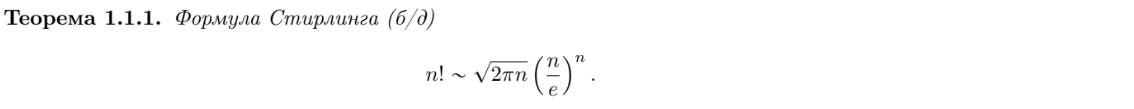
\includegraphics[width=18cm]{polina_9.PNG}\\
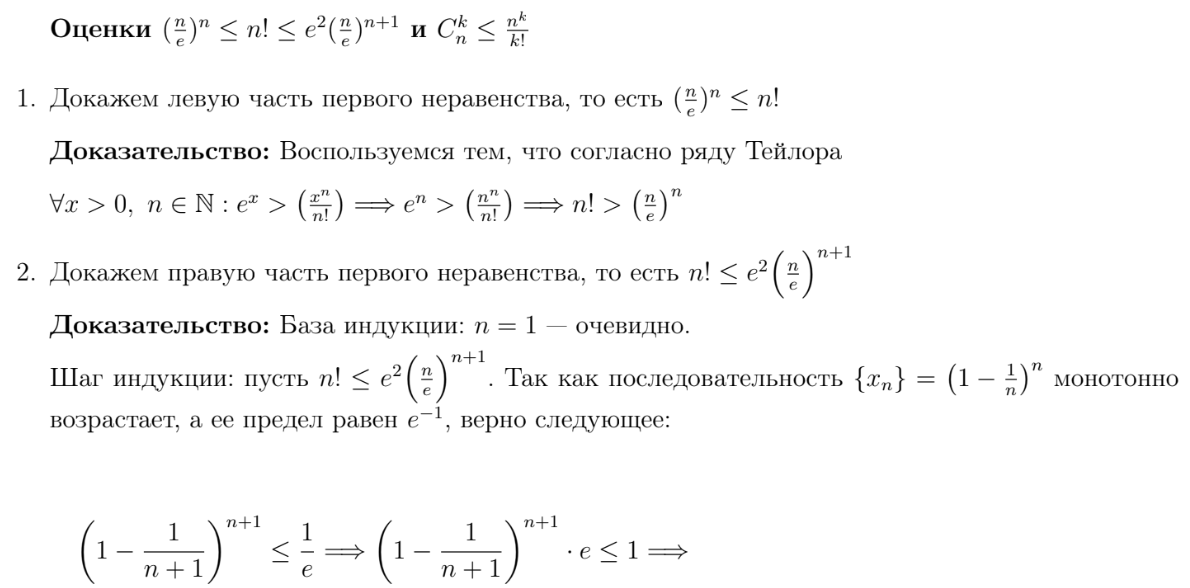
\includegraphics[width=18cm]{polina_6.PNG}\\
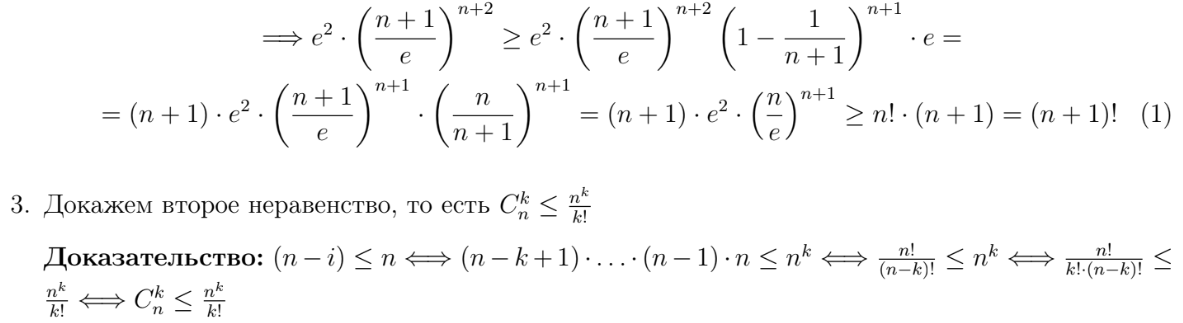
\includegraphics[width=18cm]{polina_7.PNG}\\
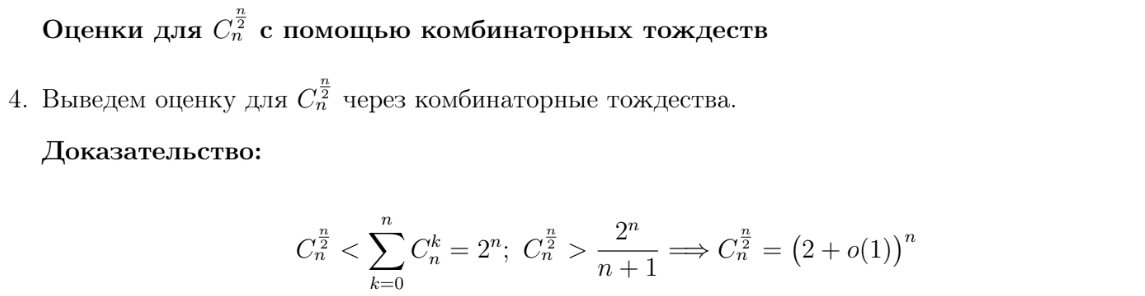
\includegraphics[width=18cm]{polina_8.PNG}
\section{(5) Асимптотика $ln (n!)$ и $\sqrt[n]{n!}$ (с доказательством без использования формулы Cтирлинга).}
\begin{itemize}
    \item [1] $\sqrt[n]{n!}$. Воспользуемся неравенством $n^ne^{-n} \leqslant n! \leqslant n^{n+1}e^{-n+1}$. Извлечём
корень n-ой степени из всех его частей и получим $\frac{n}{e} \leqslant \sqrt[n]{n!} \leqslant (ne)^{\frac{1}{n}}(\frac{n}{e})$. Заметим, что правая и левая части при $n \rightarrow \infty$ стремятся к $\frac{n}{e}$, откуда $\sqrt[n]{n!} \sim \frac{n}{e}$
\item[2] $ln (n!)$  Воспользуемся неравенством из предыдущего билета. Прологарифмируем все его части и получим $nln(n) - n\leqslant ln(n!)\leqslant (n+1)ln(n) - (n-1) \Longrightarrow ln (n!) \sim nln(n)$
\end{itemize}
\section{ (6) Оценки биномиальных коэффициентов вида $C^{[an]}_n, a \in (0, 1)$. Аналогичные результаты для полиномиальных коэффициентов}
\
\\
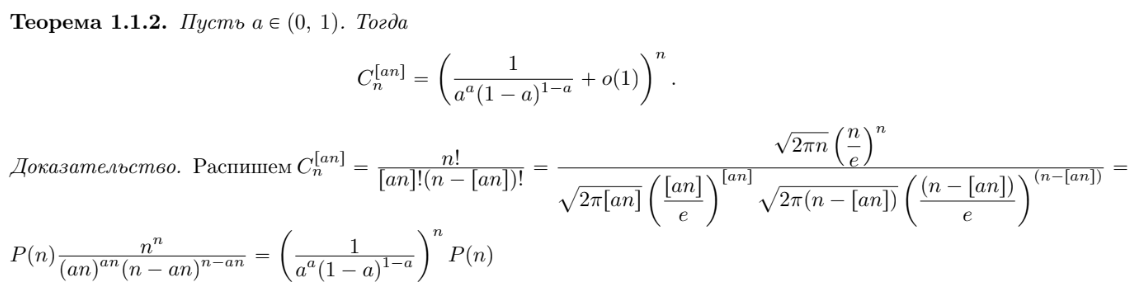
\includegraphics[width=18cm]{polina_10.PNG}\\
\includegraphics[width=18cm]{polina_11.PNG}\\
Аналогично\\
\includegraphics[width=18cm]{images/polina_12_new.PNG}
\section{(6) Асимптотика для $C_n^k$ при $k^2 = o(n)$. Оценки той же величины при больших $k$. Асимптотики для $C_{2n}^n/C_{2n}^{n-k}$.}
\
\\
\includegraphics[width=18cm]{images/polina_12.PNG}\\
$C_{2n}^n/C_{2n}^{n-k}$\\
\includegraphics[width=15cm]{images/polina_15.PNG}\\
\includegraphics[width=15cm]{images/polina_16.PNG}
\section{(5) Симметричный случай ЛЛЛ (б/д). Вывод оценки диагонального числа Рамсея (теорема Спенсера).}
\textbf{Теорема (ЛЛЛ, симметричный случай)}
\begin{itemize}
    \item [1]Пусть $A_1, ..., A_n$ - события,  $\forall i \ P(A_i) \leq p$.
    \item[2] Пусть $\forall i$ событие $A_i$ не зависит от совокупности остальных событий, кроме не более чем d штук.
    \item[3] $p < \frac{1}{e(d+1)}$. 
\end{itemize}
Тогда $P(\bigcap\limits_{i=1}^{n}\overline{A_i}) > 0$
 

\textbf{Определение} A не зависит от совокупности $B_1, ..., B_n$, если $\forall I \in \{1 ... n\} \ P(A \ |\ \bigcap\limits_{i \in I}B_i) = P(A) $

\textbf{Теорема Спенсера}
\begin{center}
Пусть для фиксированного s число n таково, что 
$e \cdot 2^{1-C_s^2}(C_{n}^{s-2}C_{s}^2) < 1$, тогда $R(s,s) > n$
\end{center}
\Proof 
 $R(s,s) > n \leftrightarrow \ \exists G$ на n вершинах, такой что 
    \begin{itemize}
        \item $w(G) < s$
        \item $\alpha(G) < s$
    \end{itemize}
    
Рассмотрим случайный граф $G(n, \frac{1}{2})$. $A_1, ..., A_{C_{n}^s}$ - все s-элементные подмножества множества вершин графа. Рассмотрим событие $E_i$ - $A_i$ образует клику или независимое множество.
\\
p = $2^{1 - C_s^2}$
\\
$d = |\{ j: |A_i \bigcap A_j| \geqslant 2\}| = \sum\limits_{t=2}^{s-1} C_s^tC_{n-s}^{s-t} < C_s^2C_{n}^{s-2}$ (справа налево. Берём две вершинки в нашем множестве $A_i$, и добиваем множество до множества размера s любыми вершинками из оставшихся, в том числе и вершинками из множества, поэтому мы учтём некоторые выбранные множества несколько раз, откуда получаем такое неравенство). Если $e \cdot 2^{1-C_s^2}(C_{n}^{s-2}C_{s}^2) < 1$, то по ЛЛЛ получаем, что найдется граф на n вершинах, в котором нет ни s-клики, ни s-независимого множества
\EndProof
\\
\textbf{Следствие}
\\
$R(s,s) \geqslant 2^{s/2}s\frac{\sqrt{2}}{e}(1+o(1))$
\\
\Proof

\includegraphics[width=18cm]{images/polina_13.PNG}

\includegraphics[width=18cm]{images/polina_14.PNG}
\EndProof
\section{(8) Симметричный и несимметричный случай ЛЛЛ (с доказательством симметричного либо напрямую, либо с доказательством несимметричного и выводом из него)}
\textbf{Определение} Пусть $A_1, ..., A_n$ - события. $G = (V,E)$ является орграфом зависимостей для этих событий, если $V = \{A_1,..., A_n\}$ и $\ \forall \ i$
\ $A_i$ не зависит от совокупности всех событий, с которыми оно не соединено исходящими ребрами
\\
\\
\textbf{ Теорема (ЛЛЛ, общий случай)} 
\\
Пусть $A_1, ..., A_n$ - события.  $G = (V,E)$ - орграф зависимостей, для которого существуют $x_1, ..., x_n \ \in [0,1): \\ \forall i \ P(A_i) \leq x_i*\prod\limits_{j: (A_i A_j) \in E}(1-x_j)$
\\
Тогда $P(\bigcap\limits_{i=1}^n \overline{A_i}) \geq \prod\limits_{j=1}^n(1-x_j) > 0$
\\
\\
\textbf{Докажем симметричный случай}
\Proof
\begin{itemize}
    \item [1] d = 0
    \\ $P(\bigcap\limits_{i=1}^n \overline{A_i}) = \prod\limits_{i=1}^n(P(\overline{A_i})) = \prod\limits_{1=1}^n(1-P(A_i)) \geq (1-p)^n \geq (1+1/e)^n > 0 $
    \item[2] $d \geq 1$ \\ $x_i = \frac{1}{d+1}$
    \\
    В качестве G возьмем такую конструкцию. Берем $A_i$ и выделяем группу из d событий, от которых $A_i$ может зависить, и проводим стрелки.
    \\
    Нам нужно доказать, что $P(A_i) \leq \frac{1}{d+1}\prod\limits_{j: (A_i, A_j) \in E}(1 - \frac{1}{d+1})$. Достаточно показать, что $p \leq \frac{1}{d+1}(1 - \frac{1}{d+1})^d$. Почему? Стрелочек, то есть ор. ребер не больше чем d, поэтому мы лишь усилили условие. С другой стороны из симметричного ЛЛЛ  $P(A_i) \leq p$. 
    \\
    Но тогда можно еще усилить условие и показать, что  $p \leq \frac{1}{d+1}\frac{1}{e}$, что известно из условия
\end{itemize}
    \EndProof
    \\
    \\
    Теперь докажем общий случай\\
    \Proof
    \\
    $P(\bigcap\limits_{i=1}^n \overline{A_i}) = P(\overline{A_1})P(\overline{A_2}|\overline{A_1})* ... * P(\overline{A_n}| \overline{A_1}\bigcap \overline{A_2} \bigcap...\bigcap \overline{A_{n-1}}) = (1 -P(A_1))(1 - P(A_2|\overline{A_1}))* ... *(1 - P(A_n| \overline{A_1}\bigcap \overline{A_2} \bigcap...\bigcap \overline{A_{n-1}}))$
    \\
    \\
    Нужно показать, что вычитаемое в i-й скобке $\leq x_i$. Тогда получим в точности утверждение теоремы. Чтобы это доказать, воспользуемся леммой ниже. Достаточно будет выбрать лишь нужное J 
    \\
    \textbf{Лемма}
\\
$\forall i \ \forall J \subset \{1,..., n\} \backslash \{i \} \ P(A_i | \bigcap\limits_{j \in J}\overline{A_j}) \leq x_i$\\
\Proof Зафиксируем i. Индукция по |J|.
\begin{itemize}
    \item [1] $|J| = 0$. В этом случае в перечесении мы получим все вероятностное пространство, в котором живут $A_j$. $\Omega \backslash \bigcup A_j = \bigcup \overline{A_j} = \Omega$, откуда $P(A_i) \leq x_i$
    \item [2] Фиксируем $J$
    \item[3]$J_1 = \{j\in J: (A_i, A_j) \in E\}$\\ $J_2 = \{j\in J: (A_i, A_j) \not \in E\}$
    \begin{itemize}
        \item[1] Пусть $J_1$ - пустое. \\ Тогда $P(A_i | \bigcap\limits_{j \in J}\overline{A_j}) = P(A_i|\bigcap\limits_{j \in J_2}\overline{A_j})$ = (в силу независимости в совокупности) $P(A_i) \leq x_i$
        \item[2] $J_1 \neq \emptyset , J_1 = \{j_1,..., j_r\} \\ P(A_i| \bigcap_{j \in J}\overline{A_j}) = \frac{P(A_i \bigcap( \bigcap\limits_{j \in J_1}\overline{A_j})| \bigcap\limits_{j \in J_2}\overline{A_j})}{P(\bigcap\limits_{j \in J_1}\overline{A_j}| \bigcap\limits_{j \in J_2}\overline{A_j})} \leq \frac{P(A_i |\bigcap\limits_{j\in J_2}\overline{A_j})}{P(\bigcap\limits_{j \in J_1}\overline{A_j}| \bigcap\limits_{j \in J_2}\overline{A_j})} \leq \frac{x_i \prod\limits_{j:(A_i, A_j) \in E} (1 - x_j)}{P(\bigcap\limits_{j \in J_1}\overline{A_j}| \bigcap\limits_{j \in J_2}\overline{A_j})}$
        \\
        Осталось показать, что $P(\bigcap\limits_{j \in J_1}\overline{A_j}| \bigcap\limits_{j \in J_2}\overline{A_j}) \geq \prod\limits_{j:(A_i, A_j) \in E} (1 - x_j)$
        \\
        \\
        $P(\bigcap\limits_{j \in J_1}\overline{A_j}| \bigcap\limits_{j \in J_2}\overline{A_j}) =
        P(\overline{A_{j_1}}| \bigcap\limits_{j \in J_2}\overline{A_j})*P(\overline{A_{j_2}}| \bigcap\limits_{j \in J_2}\overline{A_j} \bigcap A_{j_1})* ... * P(\overline{A_{j_r}}| \bigcap\limits_{j \in J_2}\overline{A_j}\bigcap \overline{A_{j_1}} ... \bigcap \overline{A_{j_{r-1}}}) \\ = (1 -P( A_{j_1}| \bigcap\limits_{j \in J_2}\overline{A_j}))(1 -P(A_{j_2}| \bigcap\limits_{j \in J_2}\overline{A_j} \bigcap \overline{A_{j_1}}))* ... * (1 -P(A_{j_r}| \bigcap\limits_{j \in J_2}\overline{A_j}\bigcap \overline{A_{j_1}} ... \bigcap \overline{A_{j_{r-1}}})) \geq \prod\limits_{j \in J_1}(1 - x_j) \geq \prod\limits_{j:(A_i, A_j) \in E}(1 - x_j)$ (Это верно, так как справа мы учитываем не только индексы из J, но и может быть другие, но при этом индексы из  J будут учтены точно)
    \end{itemize}
    \EndProof
\EndProof
\end{itemize}
\section{(8) Пример применения несимметричного случая ЛЛЛ для нижней оценки R(3, t) (вычислять оптимальные параметры не требуется). Самые точные известные оценки для R(3, t) (б/д).}

\textbf{Нижняя оценка $R(3,t)$}

Пусть G(n, p) - случайный граф \\
Рассмотрим события $A_1, ... A_{C_n^3}$ - обозанающие, что соответствующее подмножество вершин графа образует треугольник. $P(A_i) = p^3$
\\
$B_1, ... B_{C_n^t}$ - соответствующее подмножество вершин ггафа образует независимое множество на t вершинах. $P(B_i) = (1-p)^{C_t^2}$
\\
Чтобы оценить $R(3,t)$ снизу числом n, надо показать, что при данном n $P(\bigcap\limits_{i=1}^{C_n^3}(\overline{A_i})\bigcap \bigcap\limits_{j=1}^{C_n^t}(\overline{B_j})) > 0$
\\
\\
Построим граф зависимостей. Он будет иметь стрелки 4х видов:
\\
\includegraphics[]{polina_4.PNG}
\\
\begin{equation*}
\begin{cases}
   \#(A_i \rightarrow A_j) = 3(n-3)\\
  \#(A_i \rightarrow B_j) = 3C_{n-3}^{t-2} + C_{n-3}^{t-3} \\
  \#(B_i \rightarrow B_j) = C_n^t - tC_{n-1}^{t-1} - C_{n-t}^{t} \\
  \#(B_i \rightarrow A_j) = (n-t)C_t^2 + C_t^3
 \end{cases}
\end{equation*}
\\
Для Локальной Леммы Ловаса нужно, чтобы \\
$p^3 \leq x*\prod\limits_{j: (A_i, A_j)}(1-x)*\prod\limits_{j: (A_i, B_j)}(1-y)  =  x(1-x)^{\#(A_i \rightarrow A_j)}(1-y)^{\#(A_i \rightarrow B_j)}\\ (1-p)^{C_t^2} \leq y*\prod\limits_{j: (B_i, B_j)}(1-y)*\prod\limits_{j: (B_i, A_j)}(1-x)  =  y(1-y)^{\#(B_i\rightarrow B_j)}(1-x)^{\#(B_i \rightarrow A_j)}$
\\
\\
Отсюда получаем формулировку 
\\\textbf{Теоремы}
\\
\\
Пусть для данного t число n таково, что \\ $\exists p \in [0,1]\ \exists x \in[0,1) \ \exists y \in[0,1): \\ \\ 1.\ p^3 \leq x(1-x)^{\#(A_i \rightarrow A_j)}(1-y)^{\#(A_i \rightarrow B_j)}
\\
2.\ (1-p)^{C_t^2} \leq y(1-y)^{\#(B_i \rightarrow B_j)}(1-x)^{\#(B_i \rightarrow A_j)}$ \\
Тогда $R(3,t) > n$
\EndProof
\\
\\
\textbf{Теорема}
\begin{center}
    $R(3,t) \geq const*\frac{t^2}{ln^2(t)}$
\end{center}
\textbf{Теорема}
\begin{center}
    $R(3,t) \geq (1 + o(1))\frac{1}{162}\frac{t^2}{ln(t)}$
\end{center}
\textbf{Теорема}
\begin{center}
    $R(3,t) \leq (1 + o(1))\frac{t^2}{ln(t)}$
\end{center}
\textbf{Теорема}
\begin{center}
    $R(3,t) \geq (1 + o(1))\frac{t^2}{4ln(t)}$
\end{center}


% следующие темы см. FILE2.tex